\chapter{Hand-object Interaction in Virtual Environments}
\label{cha:unrealgrasp}

\begin{chapterabstract}
Interaction in virtual reality (VR) environments (e.g. grasping and manipulating virtual objects) is essential to ensure a pleasant and immersive experience. In this work, we propose a visually realistic, flexible and robust grasping system that enables real-time interactions in virtual environments. Resulting grasps are visually realistic because hand is automatically fitted to the object shape from a position and orientation determined by the user using the VR handheld controllers (e.g. Oculus Touch motion controllers). Our approach is flexible because it can be adapted to different hand meshes (e.g. human or robotic hands) and it is also easily customizable. Moreover, it enables interaction with different objects regardless their geometries. In order to validate our proposal, an exhaustive qualitative and quantitative performance analysis has been carried out. On one hand, qualitative evaluation was used in the assessment of abstract aspects, such as motor control, finger movement realism, and interaction realism. On the other hand, for the quantitative evaluation a novel metric has been proposed to visually analyze the performed grips. Performance analysis results indicate that previous experience with our grasping system is not a prerequisite for an enjoyable, natural and intuitive VR interaction experience.
\end{chapterabstract}

\minitoc

\clearpage

\section{Introduction}
\label{sec:introduction}

With the advent of affordable VR headsets such as Oculus VR/Go and HTC Vive, many works and projects are using virtual environments for different applications related to: the entertainment industry (i.e. games and 3D cinema), architectural visualizations, training/simulation (e.g. flight, driving and surgical simulators), and remote operation (e.g. robotics), among others. For these applications, the realism of the virtual environment and the user interaction with the simulated world are fundamental features to guarantee a pleasant and immersive user experience. However, developers were focused more on enhancing scenes realism, by improving existing VR technologies increasing their resolution, field of view and frame rate. This fact left in the background the development of user interactions with the virtual world. 

Allowing the user to freely explore, interact and manipulate virtual objects as in the real world is paramount for achieving a fully immersive experience. For this purpose, most of VR devices come with a pair of handheld controllers which are fully tracked in 3D space and specifically designed to enable the most basic interaction tasks (i.e. object grasping and manipulation). Nevertheless, most of the currently available VR solutions and games lack of realistic interactions with the virtual objects. This is because, interactions must be in real-time and implemented efficiently, thus a high and constant frame rate is needed in order to avoid VR sickness (visual and vestibular mismatch). Maintaining the desired 90 frames per second (FPS) in a photorealistic scene alongside complex interactions is not straightforward. This indicates the need of a flexible and efficient grasping system which allows the user to naturally and intuitively manipulate unknown objects of different geometries in real-time. Despite of the existing approaches, interaction in VR is still an open and challenging problem.

In this paper, we propose a grasping system which enables real-time object manipulation and interaction in virtual reality environments. The user is embodied in the simulated world as a virtual human or robot agent, to freely move and interact with the virtual objects using the handheld controllers (e.g. Oculus Touch motion controllers). Unlike most existing VR approaches, based exclusively on interaction with predefined objects through animations, our grasping system is capable of interacting and/or manipulating objects regardless of their geometry. This is because the virtual hand is automatically fitted to the object shape without the need of a different grip animation for each object the user is interacting with. In this way, grasp synthesis is being simplified, since we adapt the virtual hand to multiple object shapes starting from a 6D hand pose which is user predefined. 

\begin{figure}[!t]
	\centering
	\subfloat[]{\resizebox{0.49\textwidth}{!}{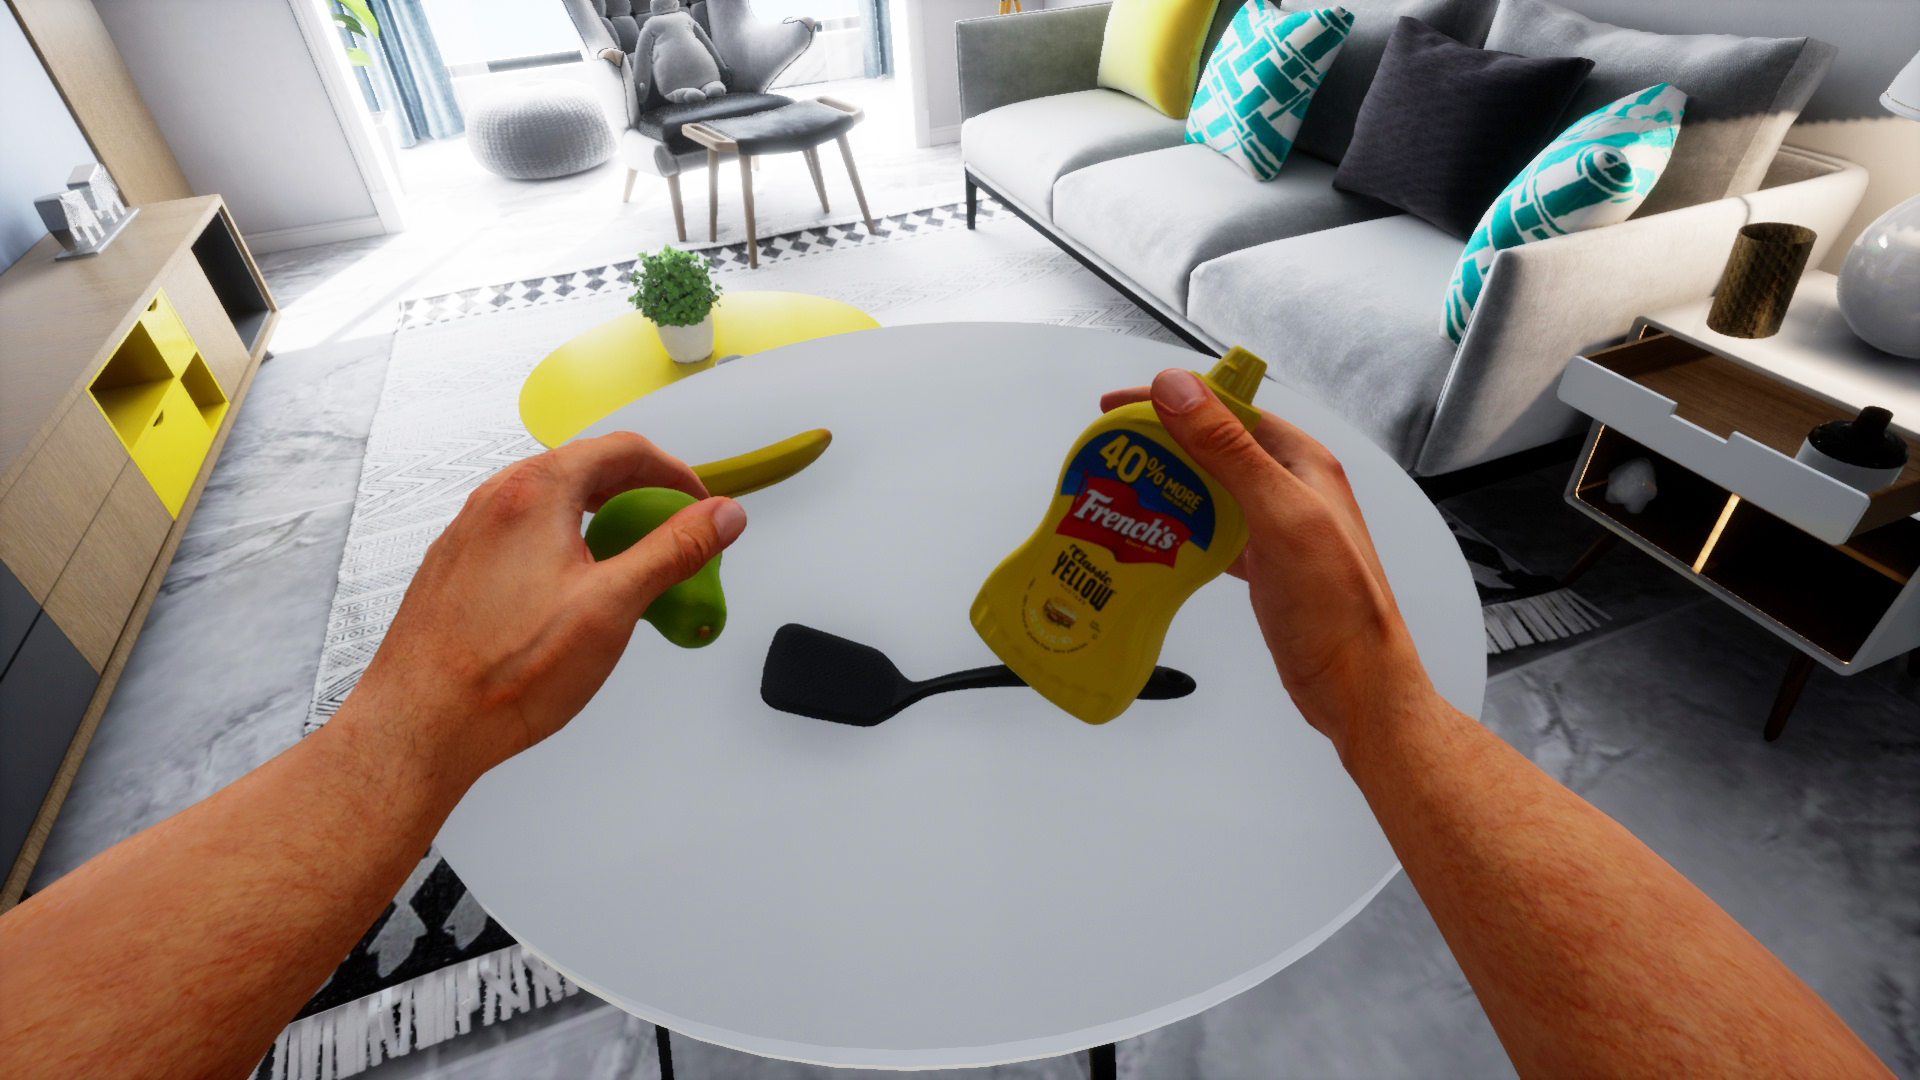
\includegraphics{figures/unrealgrasp/real_0.jpg}}
		\label{subfig:resampling_vector}}
	\subfloat[]{\resizebox{0.49\textwidth}{!}{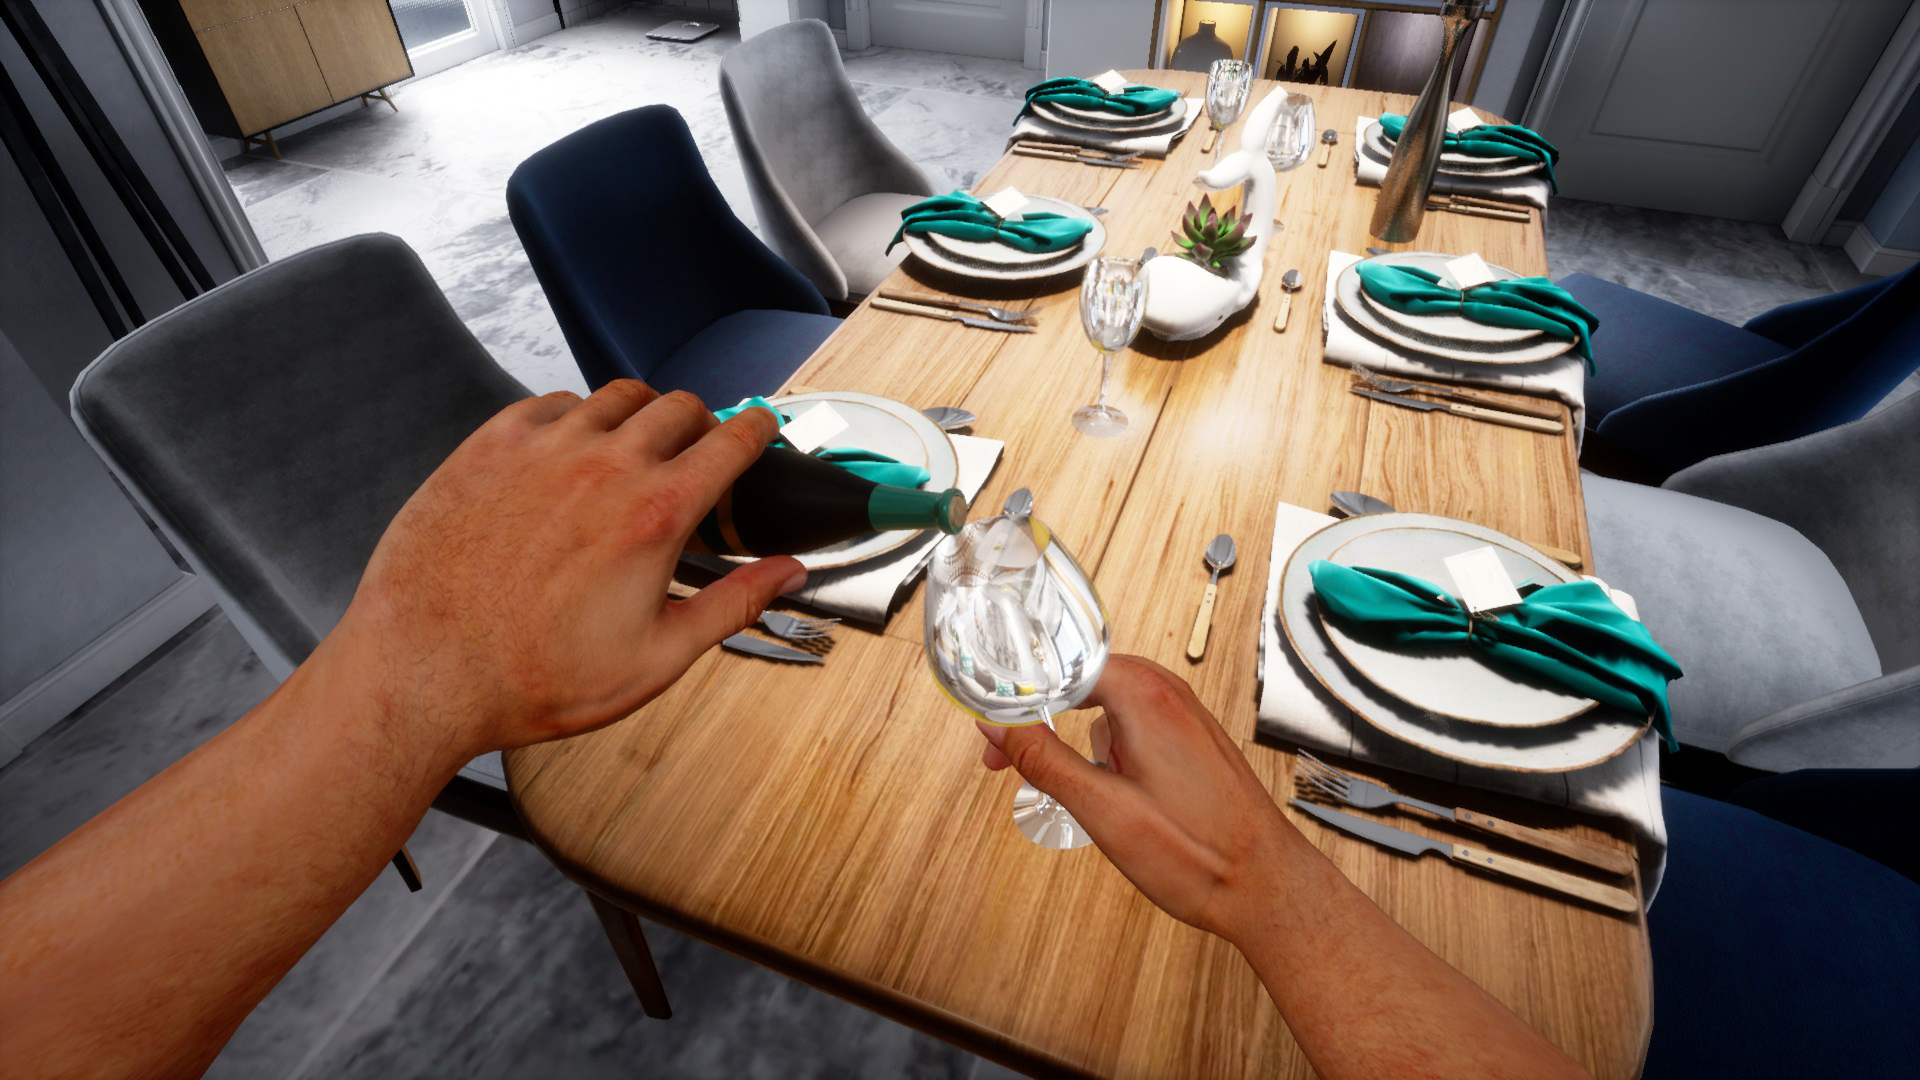
\includegraphics{figures/unrealgrasp/real_1.jpg}}
		\label{subfig:resampling_vector}}
	\\
	\subfloat[]{\resizebox{0.49\textwidth}{!}{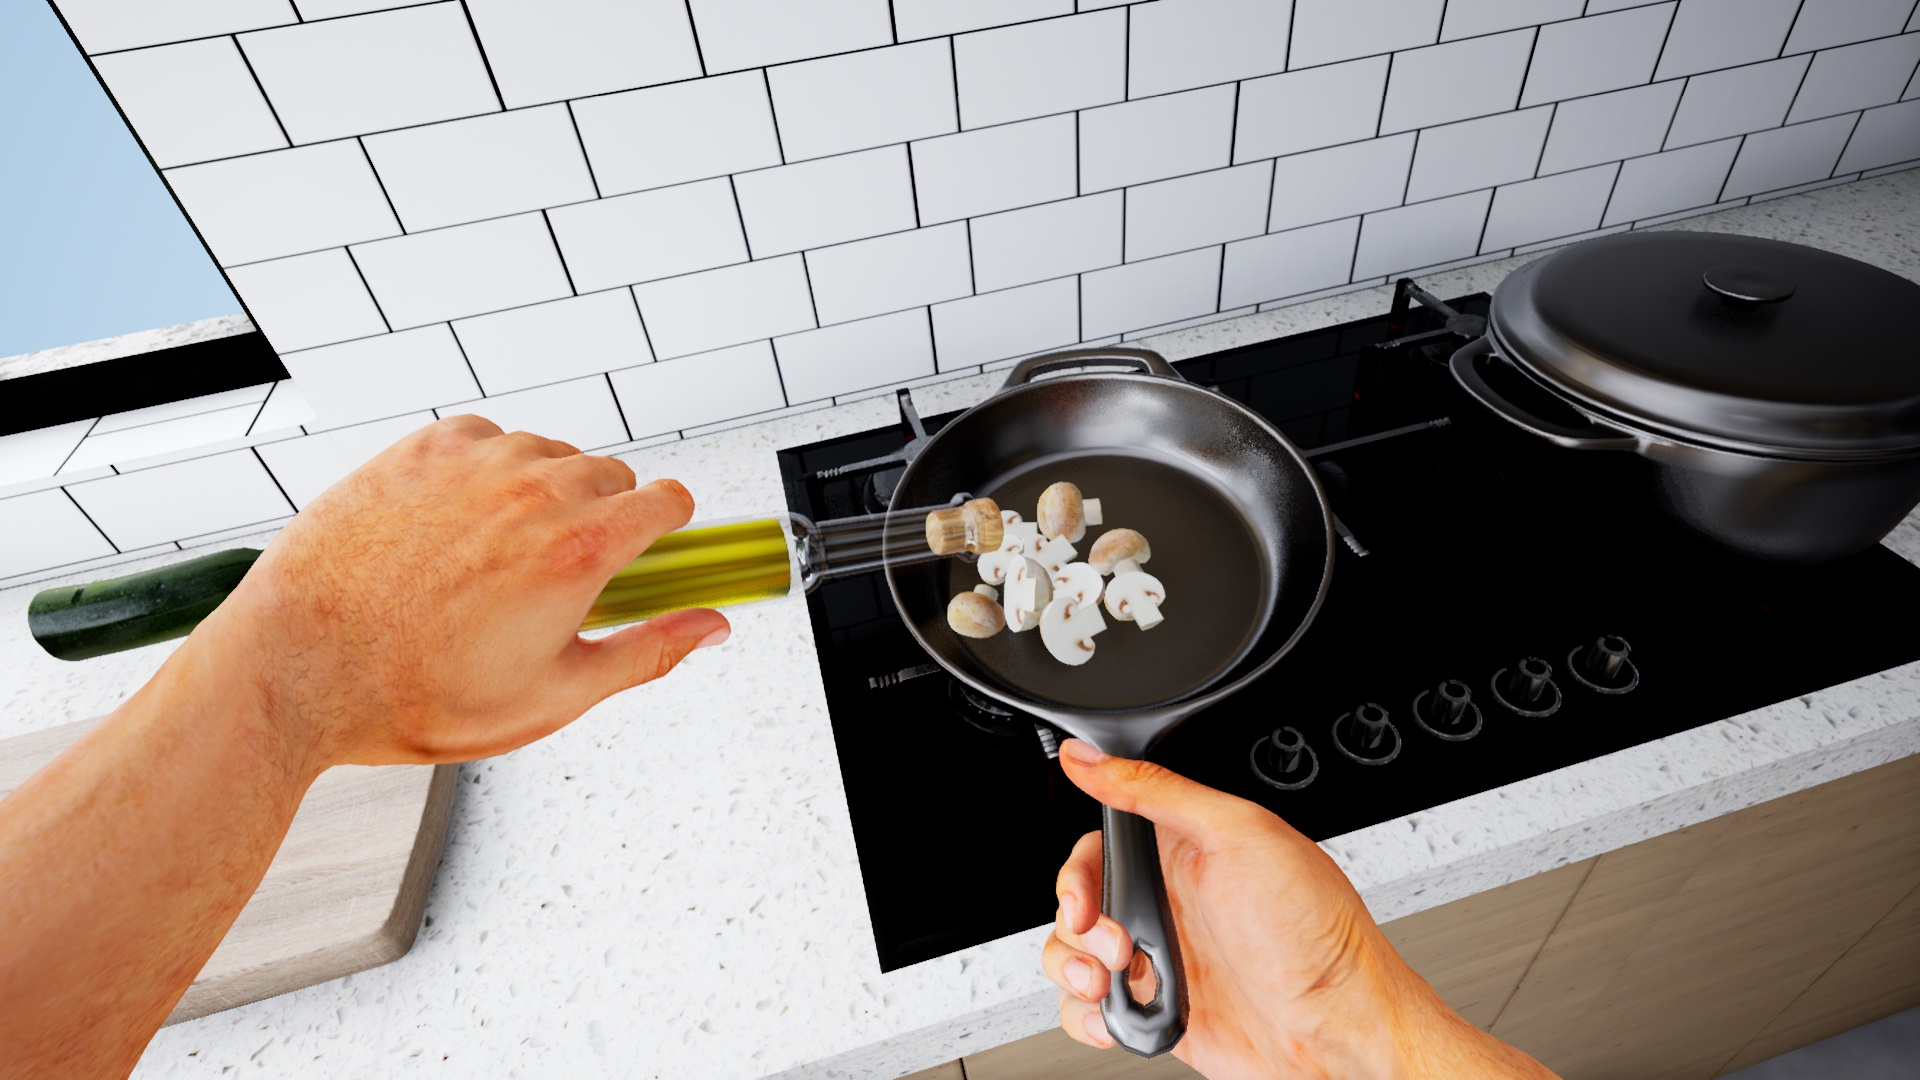
\includegraphics{figures/unrealgrasp/real_2.jpg}}
		\label{subfig:resampling_vector}}
	\subfloat[]{\resizebox{0.49\textwidth}{!}{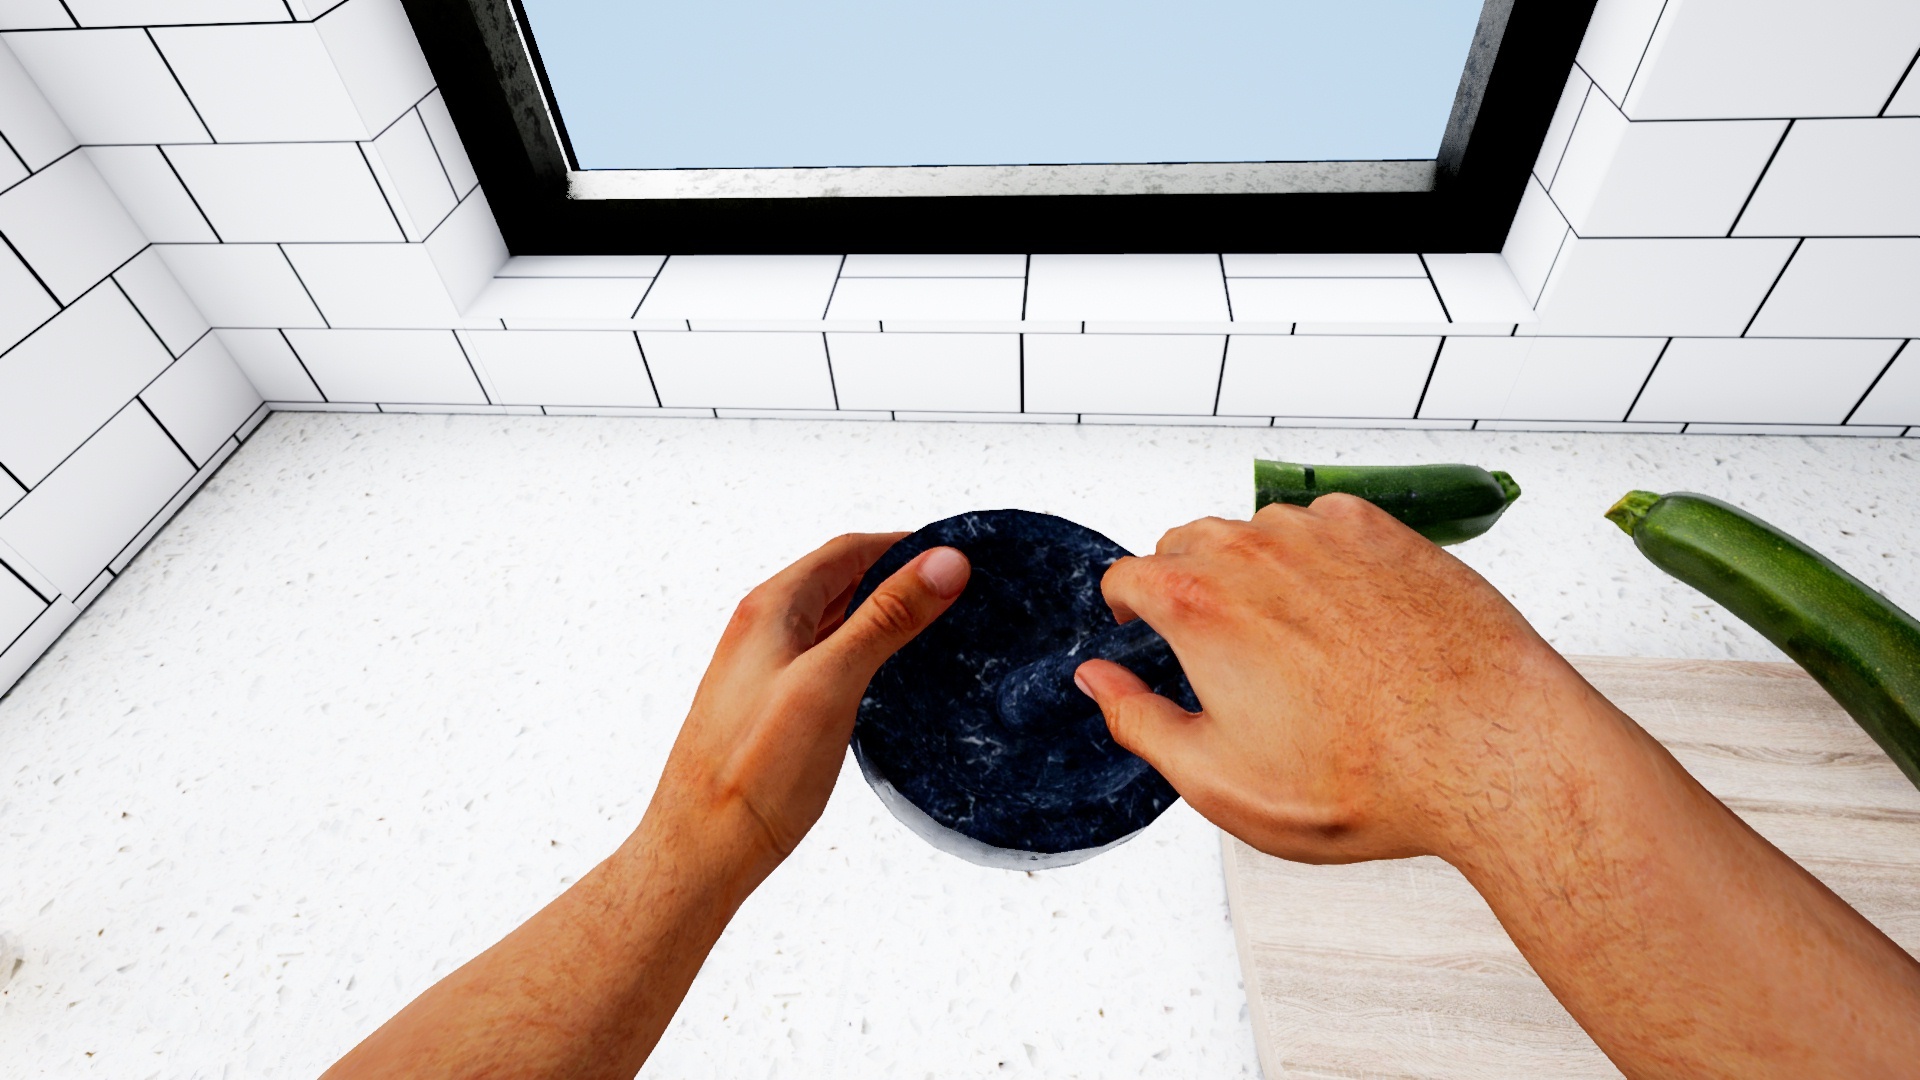
\includegraphics{figures/unrealgrasp/real_3.jpg}}
		\label{subfig:resampling_vector}}
	\caption{The user interacts with objects extracted from the YCB dataset in a photorealistic virtual environment.}
	\label{fig:interaction}
\end{figure}

Our grasping system was analyzed both qualitatively and quantitatively. On one side, for the qualitative analysis, grasping system was implemented in a photorealistic environment where the user is freely able to interact with real world objects extracted from the YCB dataset \cite{calli2015} (see Figure \ref{fig:interaction}). The qualitative evaluation is based on a questionnaire that will address the user interaction experience in terms of realism during object manipulation, system flexibility and usability, and general VR experience. On the other side, a quantitative grasping system analysis was carried out, contrasting the elapsed time a user needs in grasping an object and grasp quality based on a novel error metric which quantifies the overlapping between hand fingers and the grasped object. From the quantitative evaluation, we obtain the individual errors for the last two phalanges of each finger, the time user needed to grasp the object and also the contact points in both local and global system coordinates. The performance evaluation shows that the interaction is natural even if it is not mimicking the movement patterns of the physical world (i.e. user fingers do not close the same way as the virtual fingers). Implementation and demo videos are available at Github\footnote{\href{https://github.com/3dperceptionlab/unrealgrasp}{https://github.com/3dperceptionlab/unrealgrasp}}.

In summary, we make two main contributions:
\begin{itemize}
	\item We propose a novel, robust and flexible grasping system for real-time interactions in virtual reality environments, where hand is automatically fitted to the object shape from a 6D position determined by the user using a pair of handheld controllers;
	\item We define a novel metric and procedure to visually analyze grasping quality in VR interactions quantifying hand-object overlapping; 
\end{itemize}

The rest of the paper is structured as follows. First of all, Section \ref{sec:related_works} analyzes the latest works related to object interaction and manipulation in virtual environments. The core of this work is comprised in Section \ref{sec:graspingsystem} where our approach is described in detail. Then, the performance analysis, with the qualitative and our novel quantitative evaluations, is discussed in Section \ref{sec:experimentation}. Analysis results are reported in Section \ref{sec:results}. Then, several applications are discussed in Section \ref{sec:applications}. After that, limitations of our approach are covered in Section \ref{sec:limitationsfutureworks} alongside several feature works. Finally, some conclusions are drawn in the last Section \ref{sec:conclusion}.

\section{Related works}
\label{sec:related_works}
Grasping action is the most basic component of any interaction and it is composed of three major components \cite{aydin1999}. The first one is related to the process of approaching the arm and hand to the target object, considering the overall body movement. The second component focuses on the hand and body pre-shaping before the grasping action. Finally, the last component fits the hand to the object geometry by closing each of the fingers until contact is established.

Our work and most of the existing works related to the interaction in VR environments, are related to the third component of the grasping pipeline. Most of the existing real-time approaches are based purely on multiple predefined animations for each object the user will interact with, relying completely on the animation quality. Consequently, they are unable to deal with unknown objects without any associated predefined animation for each. This fact limits the user experience and its immersion in the VR environments by hindering their interaction capabilities.

This section contains the most recent works which are mostly aligned with our proposal where interaction is done by means of handheld controllers (e.g. Oculus VR and HTC Vive PRO controllers). In addition to these approaches, there are other interesting works considered as a valuable source of inspiration. For example, Verschoor et al. proposed a soft-hand model simulation defined as a unified energy minimization problem achieving impressive results with natural and intuitive real-time interactions \cite{Verschoor2018}. On the other hand, haptic simulation of grasping is another promising way to improve interaction in virtual environments, highlighting the work proposed by Garre et al. \cite{Garre2011}.

\subsection{Data-driven approaches}
Grasping data-driven based approaches have existed since a long time ago \cite{aydin1999}. These methods work alongside large databases containing predefined hand poses, each one associated to a concrete object geometry. The most suitable grasp pose is selected according to the defined grasp taxonomy or based on the user criteria. Most of the currently existing approaches for grasping are data-driven. The key of data-driven approaches is to effectively index large datasets in order to quickly match unknown object geometries with the most suitable hand pose from the database \cite{li2007} \cite{goldfeder2011}.

Li et al. \cite{li2007} constructed a database of hand poses for different object shapes and sizes. Despite having a good database, the process of hand pose selection was not straightforward since there can be multiple equally valid possibilities for the same object. To address this problem, Li et al. \cite{li2007} proposed a shape-matching algorithm which returns multiple potential grasp poses. The selection process is also limited by the hand high degree of freedom (DOF). In order to deal with dimensionality and redundancy many researchers have used techniques such as principal component analysis (PCA) \cite{braido2004}\cite{ciocarlie2007}. For the same purpose, Jorg et al. \cite{jorg2009} studied the correlations between hand DOFs aiming to simplify hand models reducing DOF number. 

In order to achieve realistic object interactions, other approaches also considered physical constraints \cite{pollard2005}\cite{kry2006}\cite{bai2014}. By using an initial grasp pose and a desired object trajectory, the algorithm proposed by Liu \cite{liu2009} can generate physically-based hand manipulation poses varying the contact points with the object, grasping forces and also joint configurations. Since hand and finger movement trajectories need to be both, kinematically and dynamically valid, Ye and Liu \cite{ye2012} reconstruct a realistic hand motion and grasping generating feasible contact point trajectories. 


\subsection{Virtual reality approaches}

This section is focused on the virtual reality approaches where interactions are performed using VR motion controllers, avoiding glove-based and bare-hand approaches. Implementation of the aforementioned techniques in virtual reality environments is a difficult task cause optimizations are needed to keep processes running in real-time. Most of the existing approaches for interaction in VR applications lack of realism. The existing trend is to create efficient solutions to enable real-time interactions leaving in the background interaction realism. 

Recent approaches are directly related to the entertainment industry, i.e. video games. An excellent example is \emph{Lone Echo}, a narrative adventure game which consists of manipulating tools and objects for solving puzzles. Hand animations are procedurally generated, enabling grasping of complex geometries regardless their grasp angle. This approach \cite{copenhaver2017} is based on a graph traversal heuristic which searches intersections between hand fingers and object surface mesh triangles. This is the A* heuristic, which finds the nearest palm intersections, and also filtering the invalid ones. After calculating angles to make contact with each intersection point, highest angle is selected and fingers are rotated accordingly.

Other available solutions focusing the interaction in VR are animation-based \cite{oculusDistanceGrab2017} \cite{oculusFirstExperience} \cite{vrtemplate2016}. In these approaches, user interaction with the virtual environment is limited to the objects that have a predefined grip animation. Resulting interaction is smooth and visually realistic, however it ends in a repetitive and unnatural behavior. In \cite{oculusDistanceGrab2017}, distance grab selection technique was implemented to enhance the user comfort when interacting in small play areas, while sitting or for grabbing objects on the floor. Grasping system is based on three trigger volumes attached to each hand: two small cylinders for short-range grasp, and a cone for long-range grabbing. Inspired on this approach, we adopted the usage of trigger volumes which attached to the finger phalanges we are able to control its movement and fit the hand to the object shape. 

In contrast with the available VR approaches, our system does not implement the distance grab technique (i.e. users can point to faraway objects, and have them leap into the hands when squeezing the grip button) as in \cite{oculusDistanceGrab2017}. Due to, applying our proposed performance evaluation would be not fair nor feasible. A rough comparison with similar approaches would be in terms of interaction speed, realism and naturalness. With our approach users will take longer to grasp objects as they need to previously place and orient the hand in accordance with the 6D object pose before grasping. However, these times will be increasingly shorter with practice in exchange for visually realistic results. Moreover and regarding the solution proposed in the \emph{Lone Echo} game, technical details are not sufficient to implement their proposal.


\section{Grasping system}
\label{sec:graspingsystem}

The user, embodied in the virtual environment, is able to control the position and orientation of his virtual hands using a pair of handheld controllers (for this work, the Oculus Touch and HTC Vive Pro controllers were used). These controllers are equipped with several buttons, triggers, thumbsticks and provide an accurate 6D one-to-one motion tracking. In order to grasp an object, the user would firstly position and orient the hands according to the 6D object pose and its geometry. When the hands are close enough to grasp the object, they can be closed by pressing a trigger button. In the case of Oculus Touch and HTC Vive Pro controllers, these are one-dimensional controls that report a floating point state, so the user can control the amount of closing or opening of their virtual hands (i.e. hand closing action can be stopped at any time). The system works independently of the button assigned for closing/opening action of the virtual hands, provided that it is an axis and returns floating point values depending on the amount of pressure being exerted. When closing the hand, finger movement is also conditioned by the object geometry. In other words, fingers stop moving when an overlap with the target object is detected. With this approach, hand is automatically fitted to the object shape. The user will unconsciously imitate a real human behavior when approximating his hands to grasp the virtual objects (e.g. the user will in first instance try to grab the kitchen spatula by its handle), so that the resulting interactions will be visually realistic and natural.

\subsection{Overview}
\label{subsec:overview}

Our grasping approach was designed to enable real-time interaction and manipulation in virtual reality environments by providing a simple, modular, flexible, robust, and visually realistic grasping system. Featuring an intuitive object manipulation, the interaction in VR environments results in a pleasant experience. Its main features are described as follows:

\begin{itemize}
	\item Simple and modular: system design is modular and easily customizable and extensible. All the components described in the next section can be easily modified and adapted to handle different scenarios.
	\item Flexible: our approach is flexible because it can be adapted to different hand meshes (e.g. human hand or robotic hand) without much effort. 
	\item Robust: it allows the manipulation of different objects regardless of their geometries. Most existing approaches are based on knowing or detecting the shape of the object beforehand in order to choose the best grasp from a database, or using other related techniques. Our approach enables real-time manipulation of unknown objects because hand is automatically fitted to their shapes.
	\item Visually realistic: resulting graspings are visually realistic because hand is automatically fitted to the object shape beginning from a position determined by the user using the VR handheld controllers, such as Oculus Touch or HTC Vive PRO. In other words, positioning and orienting the hand in order to grab the object is up to the user. Most of the users unconsciously would try to grasp the virtual objects such as they would be real, e.g. the user would tend to grab a hammer by its handle.
\end{itemize}

The essence of our grasping system is how the hand is automatically fitted to the object shape. The main idea behind, is to keep moving the fingers when closing the hand until a collision with the object to be grasped is detected. Through the use of trigger actors placed experimentally on the last two phalanges of each finger, we could detect when a specific finger is in contact with the manipulated object. 


\subsection{Grasp animation and trigger placement}

In order to choose the most appropriate hand closing animation we analyzed the grasp taxonomy proposed by Feix et al. \cite{feix2016grasp} in which we can find 33 different grasp types arranged according to power/precision requirements, opposition type (palm, pad or side opposition) and thumb position (abducted or adducted). On the basis of this taxonomy a common pattern has been identified in multiple power grips when manipulating objects of different geometries and sizes. This pattern is the cylindrical grasp, and it was suitable to imitate the different grips proposed in the taxonomy (e.g. power sphere, medium wrap, large diameter, etc.). This pattern is directly related to "power grasp" in which, according to Landsmeer \cite{Landsmeer1962}, the fingers and thumb wrap the object (i.e. there is a rigid relationship between the object and hand movement). In contrast, the "precision handling" is commonly used to manipulate (e.g. tip pinch) an object using the index, middle and thumb finger pads. In this case, and also for intermediate grips, several animations are needed, which implies selecting the proper animation according to the object being manipulated. However, to keep the grasping pipeline simple, we initially focused on power grasp using the cylindrical grip as a single hand closing animation.

Each grasp can be also classified according to the direction in which the hand is applying forces on the object to achieve a stable grasp. There are three basic grasping opposition types in which the direction of applied force varies:

\begin{figure}[!t]
	\centering
	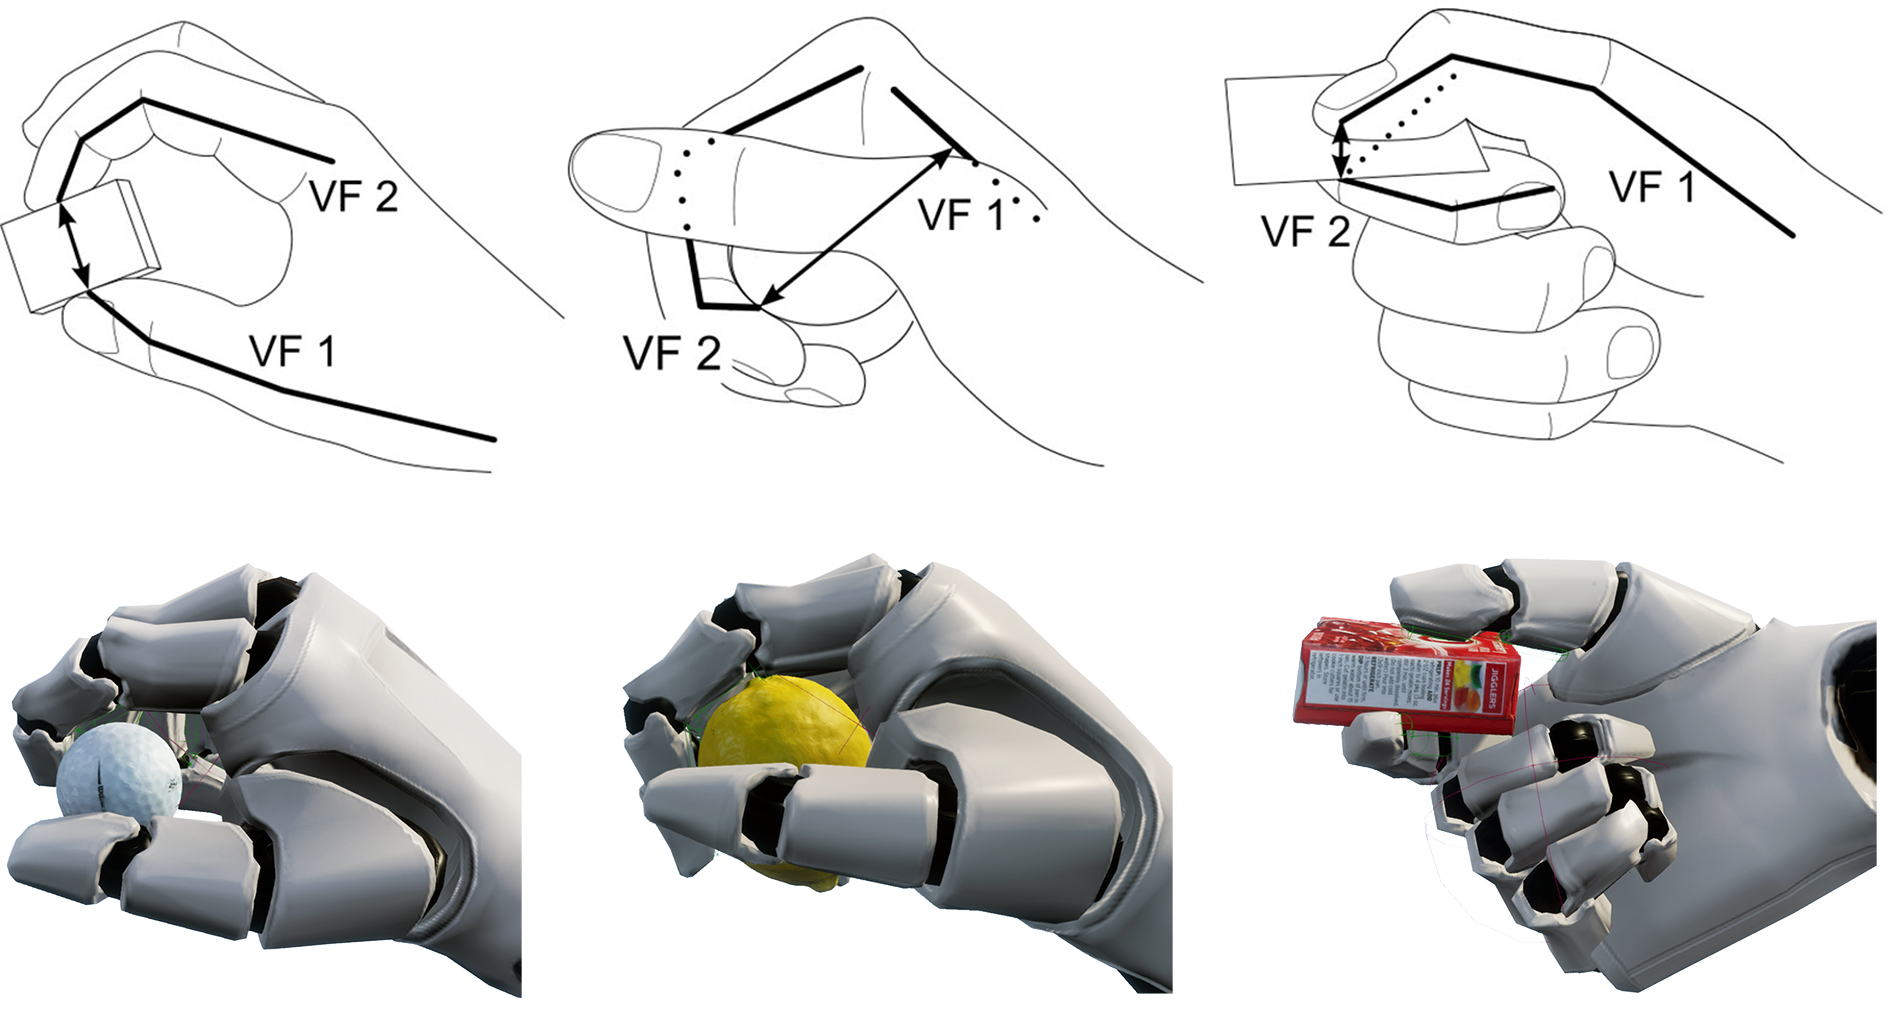
\includegraphics[width=0.95\linewidth]{figures/unrealgrasp/grasp_taxonomy.jpg}
	\caption{Represented from left to right the three different opposition types of the grasping hand: pad opposition, palm opposition, side opposition. The abbreviation VF refers to Virtual Finger. Figure adapted from \cite{feix2016grasp}.}
	\label{fig:grasp_taxonomy}
\end{figure}

\begin{itemize}
	\item Pad Opposition: force direction is usually parallel to hand palm. This opposition type is commonly used in precision grips which are performed using palmar surface and fingertips. This is represented in Figure \ref{fig:grasp_taxonomy} (bottom left) where a golf ball is attempted to be grasped using thumb and index fingertips. Regarding the grasp performed using our grasping system, it not represent an accurate "pinch" grasp. This is mainly because the closing hand animation was designed specifically for power grasp, performing worse in precision handling.
	\item Palm Opposition: commonly used in power grip, where forces on the object are mostly perpendicular to the palm and fingers wrap the object. As we can see in the Figure \ref{fig:grasp_taxonomy}, the lemon is accurately grasped between all the fingers and palmar surface, indicating that our approach was designed for power grip using palm opposition.
	\item Side Opposition: forces on the object are commonly applied transversally to the palm of the hand. With our virtual hand configuration and the capsule trigger placement, we can only detect overlapping at the fingertips. Consequently, our approach is not able to effectively perform side opposition grips. For a lateral grasp, we would have to change the size of the capsule triggers so that they stand out on the sides, or, place other triggers on the finger sides, thus increasing the complexity of our grasping system. In the Figure \ref{fig:grasp_taxonomy} (bottom right), the capsule trigger placed on the distal index phalanx is slightly in contact with the box, thus a lateral grip is possible. However, it is not straightforward to replicate this situation.	
\end{itemize}



\subsection{Trigger placement}

\begin{figure}[!t]
	\centering
	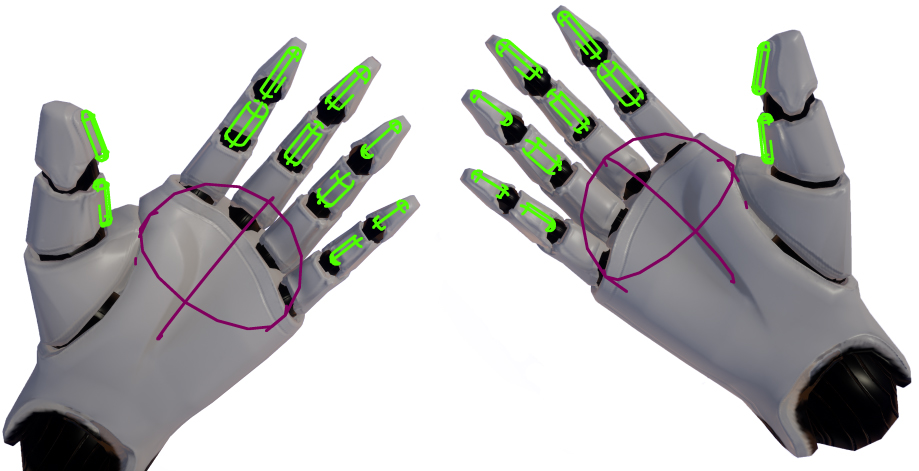
\includegraphics[width=.8\linewidth]{figures/unrealgrasp/mannequin_hands.jpg}
	\caption{Represented in green, the capsule triggers of the middle and distal phalanges. In purple, sphere trigger of the palm used to detect the nearest object to be grasped.}
	\label{fig:mannequinhands}
\end{figure}

A trigger actor is a component from Unreal Engine 4, and other engines such as Unity, used for casting an event in response to an interaction, e.g. when the trigger overlaps an object. Trigger placement on finger phalanges was done experimentally during the interaction with objects of varied geometry from the YCB dataset. This experimentation consisted mainly on determining the number of triggers to achieve a good behavior when interacting with different sized objects and varied shapes. Trigger overlapping is checked for each frame, thus using a large number of triggers would harm system performance. Due to, trigger number has been increased progressively during the experimentation. Firstly, interaction with small and different shaped objects (e.g. cubes, spheres, cones, etc.) was performed only using triggers on the distal phalanges. The results were convincing, however, when dealing with larger objects, they were slippery in the hand until the distal triggers made contact with the object. This slippery behavior was due to the fact that the middle phalanges collided with the object before the distal ones, so the solution was to add triggers to the middle phalanges to stop their movement when overlapping with the object. Finally, a sphere trigger has been added to the hand palm in order to use the palmar surface when grasping, such as in pad and palm oppositions. This has improved interaction with small objects. The final hand configuration is represented in Figure \ref{fig:mannequinhands}.

\subsection{Grasping pipeline components}


\definecolor{lightgreen}{RGB}{166,196,138}
\definecolor{lightblue}{RGB}{143,184,237}

\tikzstyle{block} = [rectangle, draw, fill=lightgreen, 
text width=5em, text centered, rounded corners, minimum height=3em]
\tikzstyle{cloud} = [draw, ellipse, text centered, fill=lightblue, text width=4em,
minimum height=2em]
\tikzstyle{line} = [draw, -latex']

\begin{figure}[!t]
	\centering
	\resizebox{0.7\textwidth}{!}{
		\begin{tikzpicture}[node distance = 3.0cm, auto]
		% Place nodes
		\node [block] (init) {Object selection};
		\node [block, right of= init] (manager) {Interaction manager};
		\node [block, right of= manager] (movement) {Finger movement};
		\node [block, right of= movement] (logic) {Grasping logic};
		
		% Draw edges
		\path [line] (init) -- (manager);
		\path [line] (manager) -- (movement);
		\path [line] (movement) -- (logic);
		\end{tikzpicture}}$  $
	\caption{Pipeline with the components of our grasping system.}
	\label{fig:pipeline}
\end{figure}

Our grasping system is composed of the components shown in the Figure \ref{fig:pipeline}. They are defined as follows:
\begin{itemize}
	\item Object selection: selects the nearest object to the hand palm. Graspable area is determined by a sphere trigger placed on the hand palm (red colored in Figure \ref{fig:mannequinhands}). The sphere trigger returns the world location of all the overlapped actors. As a result, the nearest actor can be determined by computing the distance from each overlapped actor to the center of the sphere trigger. Smallest distance will determine the nearest object.
	\item Interaction manager: manages the capsule triggers attached to the finger phalanges as represented in Figure \ref{fig:mannequinhands}. If a capsule trigger reports an overlap event, the movement of its corresponding phalanx is blocked until hand is reopened or the overlapping with the manipulated object is over. The phalanx state (represented as a boolean value, blocked or released) will be used as input to the grasping logic component and determines when the phalanx is movable. A phalanx is defined as blocked when its attached capsule trigger is overlapping with the object being manipulated. In other words, this indicates which phalanges are in contact with the object.
	\item Finger movement: this component controls the movement of the fingers during the hand closing and opening animations. It ensures a smooth animation avoiding unexpected and unrealistic behavior during finger movement caused neither by a performance drop or other interaction issues. Basically, it monitors the variation in the movement of each phalanx. When detecting an unexpected variation, i.e. the difference in the phalanx movement during a frame change is bigger than a threshold value, missing intermediate values will be interpolated so as to keep finger movement smooth. 
	\item Grasping logic: this component decides when to grab or release an object. The decision is made based on the phalanx state provided by the interaction manager component, e.g. at least a phalanx of the thumb and index fingers need to be in contact with the manipulated object in order to perform a top pinch grasp. 
	
	The object is grasped or released according to the following function which operates using boolean values as inputs indicating when finger phalanges are in contact or not with the object:
	
	\begin{equation} \label{eq:3}
	f(th_{ph}, in_{ph}, mi_{ph}, palm)= 
	\begin{cases}
	true, & \text{if } (th_{ph} \lor palm) \\
	& \land (in_{ph} \lor mi_{ph})\\
	false,              & \text{otherwise}
	\end{cases}
	\end{equation}, where $th_{ph}$, $in_{ph}$, and $mi_{ph}$ are defined as
	
	\begin{equation} \label{eq:4}
	\begin{array}{l}
	th_{ph} = thumb_{mid} \lor thumb_{dist} \\
	in_{ph} = index_{mid} \lor index_{dist} \\
	mi_{ph} = middle_{mid} \lor middle_{dist} \\
	\end{array}
	\end{equation}
	
	Equation \ref{eq:3} determines when an object is grasped or released based on the inputs determined in Equation \ref{eq:4} and palm trigger state. $th_{ph}$, $in_{ph}$, and $mi_{ph}$, represent the OR logic operator between their middle and distal phalanges values, respectively. In other words, this indicates it is enough to detect contact only with one of the two phalanges to state that the finger is interacting with the object (e.g. thumb finger is interacting with an object when a contact with the distal or middle phalanx is detected). According to human hand morphology, $mid$ and $dist$ subscripts refer to the middle and distal phalanx (e.g. $thumb_{dist}$ references the distal phalanx of thumb finger and at the implementation level it is a boolean value).
\end{itemize}


\subsection{Implementation details}

Grasping system has been originally implemented in Unreal Engine 4 (UE4), however, it can be easily implemented in other engines such as Unity, which would also provide us with the necessary components for replicating the system (e.g. overlapping triggers). The implementation consists of UE4 blueprints and has been correctly structured in the components depicted in Figure \ref{fig:pipeline} and described in the previous section. Implementation is available at Github (\url{https://github.com/3dperceptionlab/unrealgrasp}) using different UE4 versions.

\section{Performance analysis}
\label{sec:experimentation}

In order to validate our proposal, a complete performance analysis has been carried out. This analysis covers from a qualitative evaluation, which is prevalent in the assessment of VR systems, to a novel quantitative evaluation. Evaluation methods are briefly described as follows:
\begin{itemize}
	\item Qualitative evaluation: based on the user experience interacting with real objects from the YCB dataset in a photorealistic indoor scenario. Its purpose is to assess interaction realism, immersion, hand movement naturalness and other qualitative aspects described in Table \ref{table:questionnaire} from the Subsection \ref{subsec:qualitative}, which addresses qualitative evaluation in detail.
	\item Quantitative evaluation: based on the grasping quality in terms of realism (i.e. how much it is visually plausible). We consider a visually plausible grasp when hand palm or fingers are level with the object surface, as in a real life grasping. However, when dealing with complex meshes, the collision detection precision can be significantly influenced. In this case, fingers could penetrate the object surface, or remain above its surface when a collision was detected earlier than expected. This would result in an unnatural and unrealistic grasp. To visually quantify grasping quality, we propose a novel error metric based on computing the distance from each capsule trigger to the nearest contact point on the object surface. Quantitative evaluation and the proposed error metric are addressed in detail in Subsection \ref{subsec:quantitative}.
	
\end{itemize}


\subsection{Participants}

For the performance analysis, we recruited ten participants (8M/2F) from the local campus. Four of them have previous experience with VR applications (they have already used Oculus VR and HTC Vive headsets for gaming and/or developing purposes), as well as some of them may have previous experience using our system. The rest are inexperienced users, using a VR headset for the first time. Participants will take part on both qualitative and quantitative evaluation. The performance analysis procedure will be described in the following subsection, indicating the concrete tasks to be performed by each participant.

\subsection{Dataset}

To benchmark our grasping system we used a set of objects that are frequently used in daily life, such as, food items (cracker box, cans, box of sugar, fruits, etc.), tool items (power drill, hammer, screwdrivers, etc.), kitchen items (eating utensils) and also spherical shaped objects (tennis ball, racquetball, golf ball, etc.). Yale-CMU-Berkeley (YCB) Object and Model set \cite{calli2015} provides us these real-life 3D textured models scanned with outstanding accuracy and detail. Available objects have a wide variety of shapes, textures and sizes as we can see in Figure \ref{fig:ycbgrasps}. The advantage of using real life objects is that the user already has a previous experience manipulating similar objects so he will try to grab and interact with the objects in the same way.

\begin{figure}[!t]
	\centering
	\subfloat[Master Chef can]{\resizebox{0.24\textwidth}{!}{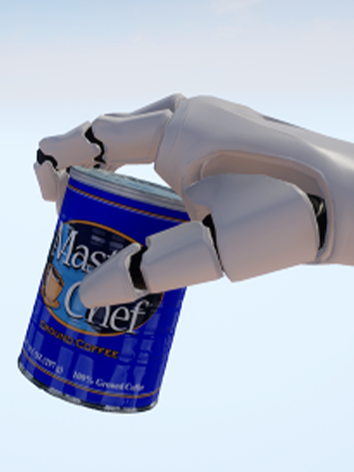
\includegraphics{figures/unrealgrasp/0.png}}
		\label{fig:masterchefcan}}
	\subfloat[Cracker box]{\resizebox{0.24\textwidth}{!}{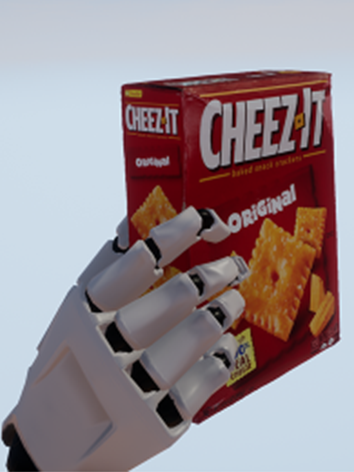
\includegraphics{figures/unrealgrasp/1.png}}
		\label{fig:crackerbox}}
	\subfloat[Sugar box]{\resizebox{0.24\textwidth}{!}{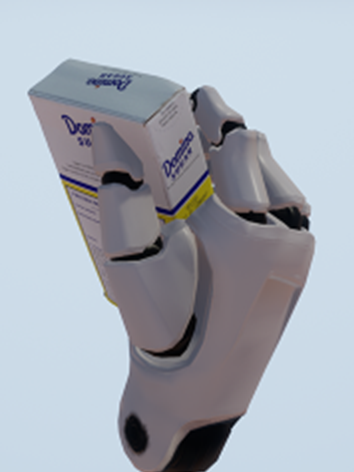
\includegraphics{figures/unrealgrasp/2.png}}
		\label{fig:sugarbox}}
	\subfloat[Tomato soup can]{\resizebox{0.24\textwidth}{!}{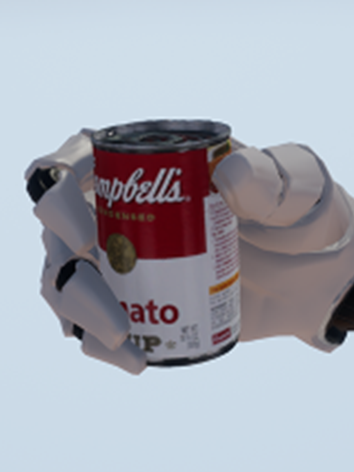
\includegraphics{figures/unrealgrasp/3.png}}
		\label{fig:tomatosoupcan}}
	\\
	\subfloat[Moustard bottle]{\resizebox{0.24\textwidth}{!}{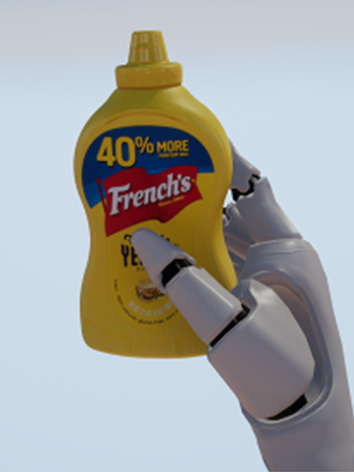
\includegraphics{figures/unrealgrasp/4.png}}
		\label{fig:mustardbottle}}
	\subfloat[Tuna fish can]{\resizebox{0.24\textwidth}{!}{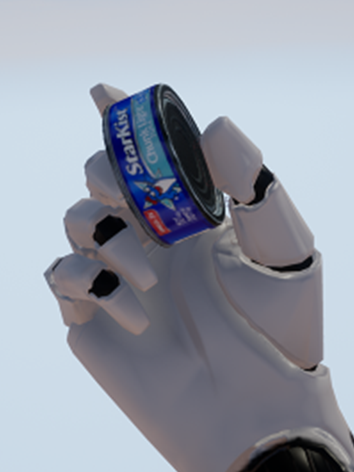
\includegraphics{figures/unrealgrasp/5.png}}
		\label{fig:tunafishcan}}
	\subfloat[Gelatin box]{\resizebox{0.24\textwidth}{!}{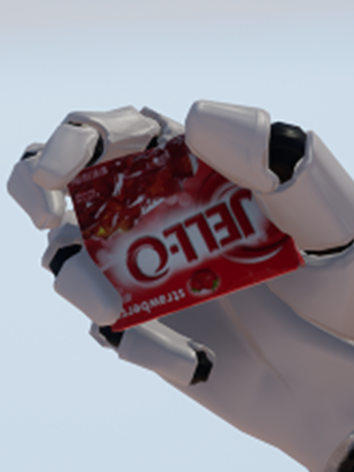
\includegraphics{figures/unrealgrasp/7.png}}
		\label{fig:gelatinbox}}
	\subfloat[Potted meat can]{\resizebox{0.24\textwidth}{!}{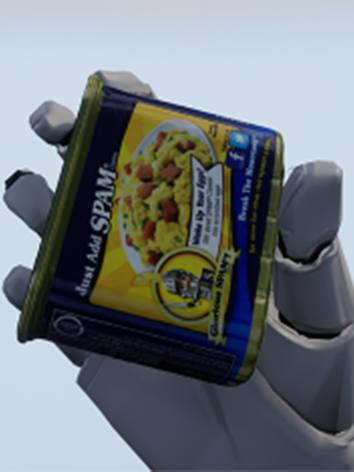
\includegraphics{figures/unrealgrasp/8.png}}
		\label{fig:pottedmeatcan}}
	\\
	\subfloat[Banana]{\resizebox{0.24\textwidth}{!}{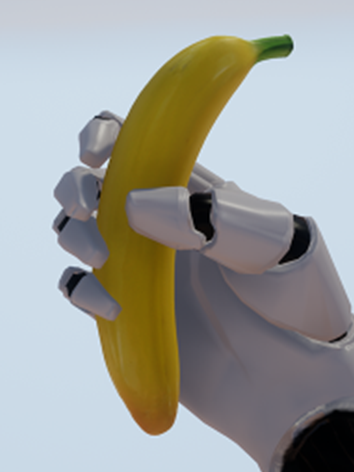
\includegraphics{figures/unrealgrasp/9.png}}
		\label{fig:banana}}
	\subfloat[Strawberry]{\resizebox{0.24\textwidth}{!}{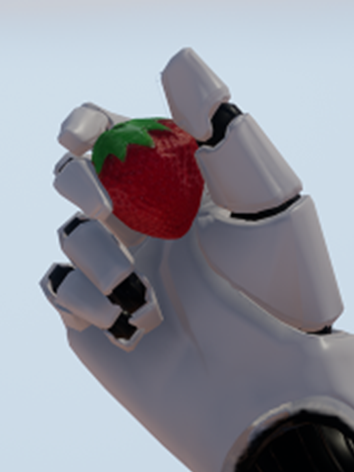
\includegraphics{figures/unrealgrasp/10.png}}
		\label{fig:strawberry}}
	\subfloat[Apple]{\resizebox{0.24\textwidth}{!}{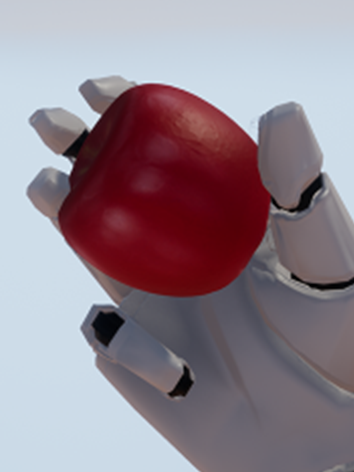
\includegraphics{figures/unrealgrasp/11.png}}
		\label{fig:apple}}
	\subfloat[Lemon]{\resizebox{0.24\textwidth}{!}{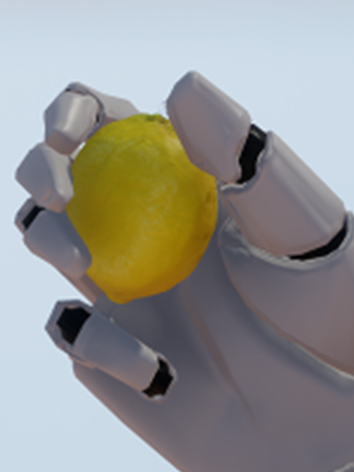
\includegraphics{figures/unrealgrasp/12.png}}
		\label{fig:lemon}}
	\\
	\subfloat[Peach]{\resizebox{0.24\textwidth}{!}{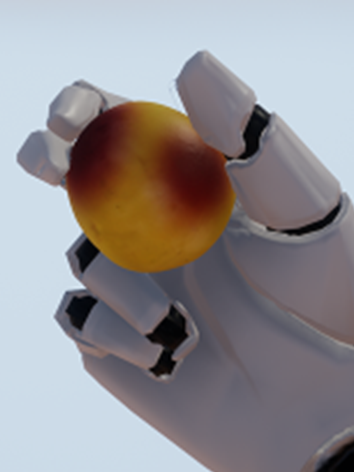
\includegraphics{figures/unrealgrasp/13.png}}
		\label{fig:peach}}
	\subfloat[Pear]{\resizebox{0.24\textwidth}{!}{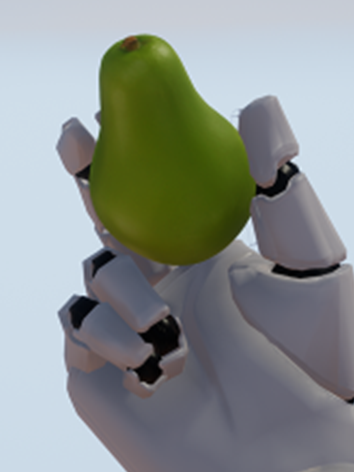
\includegraphics{figures/unrealgrasp/14.png}}
		\label{fig:pear}}
	\subfloat[Orange]{\resizebox{0.24\textwidth}{!}{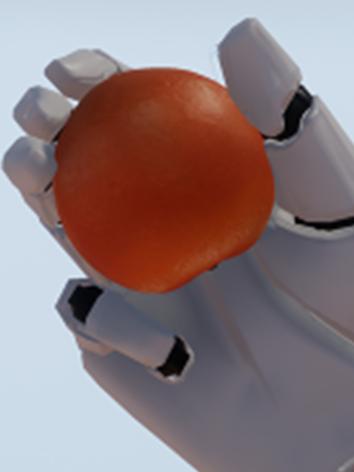
\includegraphics{figures/unrealgrasp/15.png}}
		\label{fig:orange}}
	\subfloat[Plum]{\resizebox{0.24\textwidth}{!}{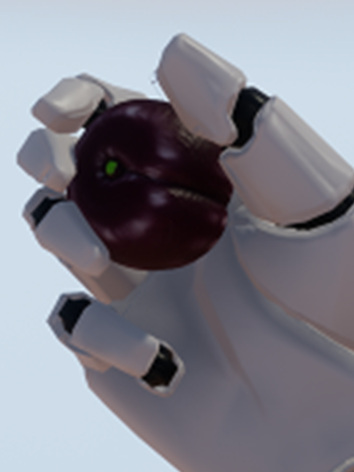
\includegraphics{figures/unrealgrasp/16.png}}
		\label{fig:plum}}
	\caption{Grasping performed on objects from the YCB dataset.}\label{fig:ycbgrasps}
\end{figure}

\begin{figure}[!t]
	\ContinuedFloat
	\centering
	\subfloat[Bleach cleaner]{\resizebox{0.24\textwidth}{!}{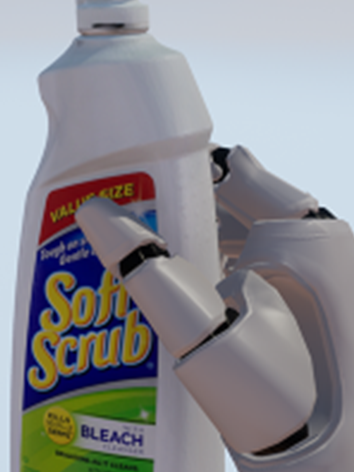
\includegraphics{figures/unrealgrasp/17.png}}
		\label{fig:bleachcleaner}}
	\subfloat[Fork]{\resizebox{0.24\textwidth}{!}{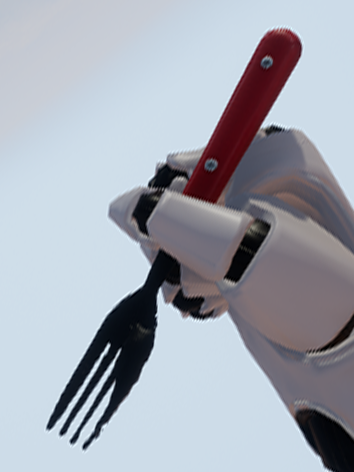
\includegraphics{figures/unrealgrasp/18.png}}
		\label{fig:fork}}
	\subfloat[Spoon]{\resizebox{0.24\textwidth}{!}{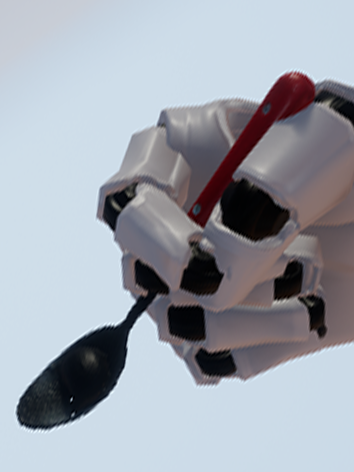
\includegraphics{figures/unrealgrasp/19.png}}
		\label{fig:spoon}}
	\subfloat[Knife]{\resizebox{0.24\textwidth}{!}{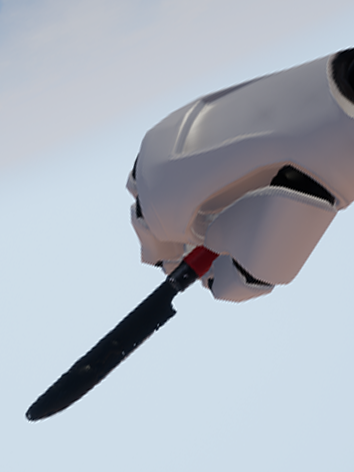
\includegraphics{figures/unrealgrasp/20.png}}
		\label{fig:knife}}
	\\
	\subfloat[Spatula]{\resizebox{0.24\textwidth}{!}{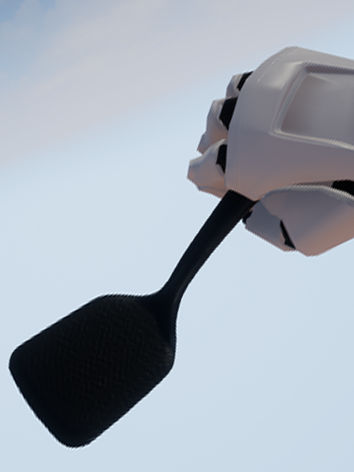
\includegraphics{figures/unrealgrasp/21.png}}
		\label{fig:spatula}}
	\subfloat[Power drill]{\resizebox{0.24\textwidth}{!}{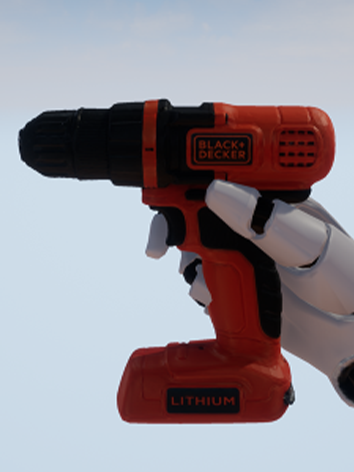
\includegraphics{figures/unrealgrasp/22.png}}
		\label{fig:powerdrill}}
	\subfloat[Scissors]{\resizebox{0.24\textwidth}{!}{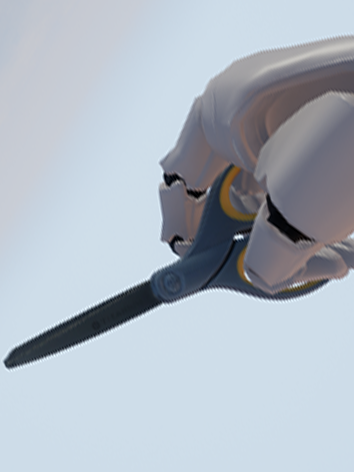
\includegraphics{figures/unrealgrasp/23.png}}
		\label{fig:scissors}}
	\subfloat[Large marker]{\resizebox{0.24\textwidth}{!}{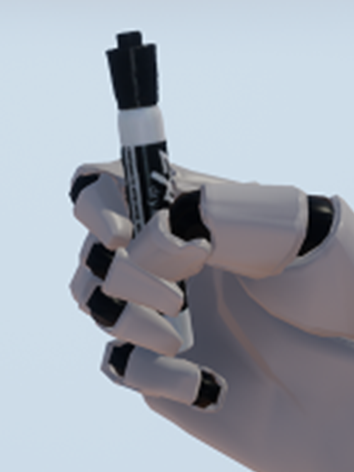
\includegraphics{figures/unrealgrasp/24.png}}
		\label{fig:largemarker}}
	\\
	\subfloat[Adjustable wrench]{\resizebox{0.24\textwidth}{!}{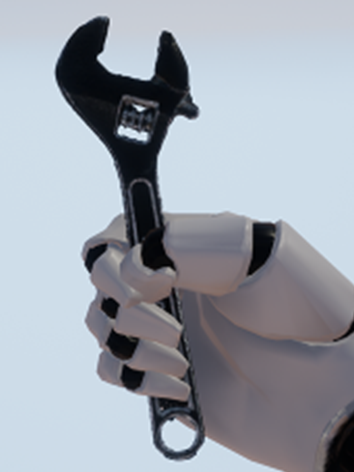
\includegraphics{figures/unrealgrasp/25.png}}
		\label{fig:adjustablewrench}}
	\subfloat[Flat screwdriver]{\resizebox{0.24\textwidth}{!}{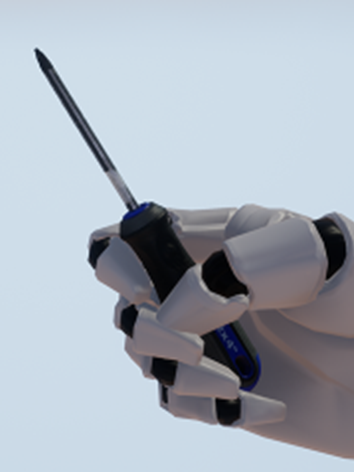
\includegraphics{figures/unrealgrasp/26.png}}
		\label{fig:flatscrewdriver}}
	\subfloat[Hammer]{\resizebox{0.24\textwidth}{!}{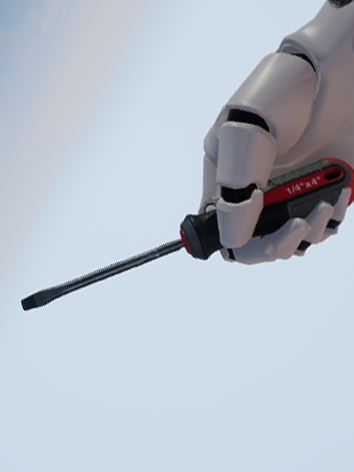
\includegraphics{figures/unrealgrasp/27.png}}
		\label{fig:hammer}}
	\subfloat[Baseball]{\resizebox{0.24\textwidth}{!}{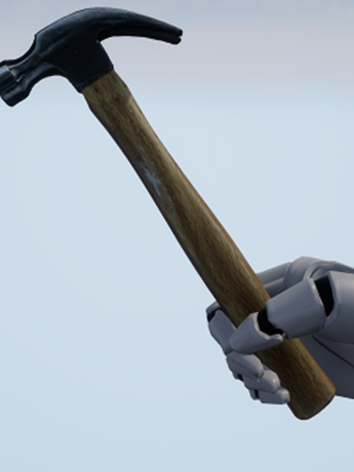
\includegraphics{figures/unrealgrasp/28.png}}
		\label{fig:baseball}}
	\\
	\subfloat[Tennis ball]{\resizebox{0.24\textwidth}{!}{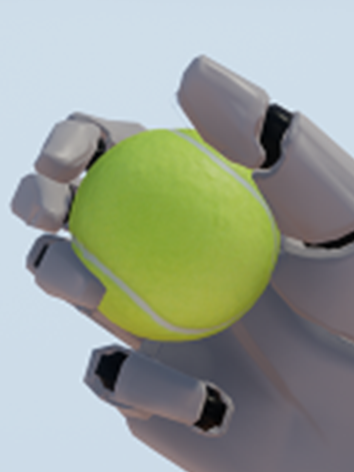
\includegraphics{figures/unrealgrasp/30.png}}
		\label{fig:tennisball}}
	\subfloat[Toy plane]{\resizebox{0.24\textwidth}{!}{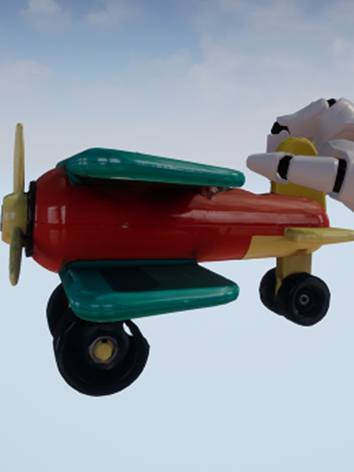
\includegraphics{figures/unrealgrasp/34.png}}
		\label{fig:toyplane}}
	\subfloat[Toy brick]{\resizebox{0.24\textwidth}{!}{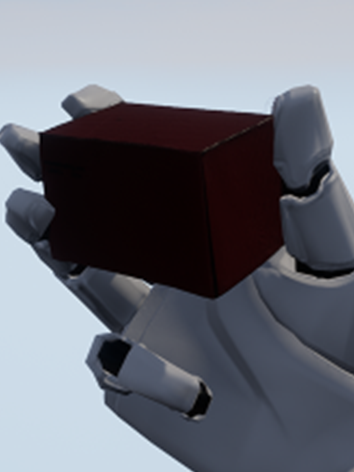
\includegraphics{figures/unrealgrasp/33.png}}
		\label{fig:toybrick}}
	\subfloat[Golf ball]{\resizebox{0.24\textwidth}{!}{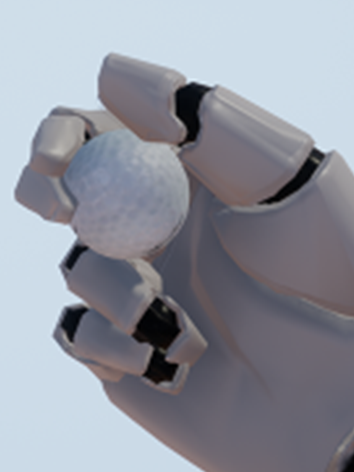
\includegraphics{figures/unrealgrasp/32.png}}
		\label{fig:golfball}}
	\caption{Grasping performed on objects from the YCB dataset.}\label{fig:ycbgrasps}
\end{figure}

\subsection{Qualitative evaluation}
\label{subsec:qualitative}

Most of VR experiments include qualitative and quantitative studies to measure its realism and immersion. Arguably, questionnaires are the default method to qualitatively assess any experience and the vast majority of works include them in one way or another \cite{Christopoulos2018} \cite{Koutsabasis2018} \cite{Vosinakis2018}. However, one of the main problems with them is the absence of a standardized set of questions for different experiences that allows for fair and easy comparisons. The different nature of the VR systems and experiences makes it challenging to find a set of evaluation questions that fits them all. Following the efforts of \cite{Gonzalez-Franco2018} towards a standardized embodiment questionnaire, we analyzed several works in the literature \cite{Poeschl2013} \cite{Brackney2017} that included questionnaires to assess VR experiences to devise a standard one for virtual grasping systems. Inspired by such works, we have identified three main types of questions or aspects:
\begin{itemize}
	\item Motor Control: this aspect considers the movement of the virtual hands as a whole and its responsiveness to the virtual reality controllers. Hands should move naturally and their movements must be caused exactly by the controllers without unwanted movements and without limiting or restricting real movements to adapt to the virtual ones.
	\item Finger Movement: this aspect takes the specific finger movement into account. Such movements must be natural and plausible. Moreover, they must react properly to the user's intent.
	\item Interaction Realism: this aspect is related to the interaction of the hand and fingers with objects. 
\end{itemize}

The questionnaire, shown in Table \ref{table:questionnaire}, is composed of fourteen questions related to the previously described aspects.
\begin{table}[!t]
	\resizebox{\linewidth}{!}{
		\begin{tabular}{cl}
			\hline
			\textbf{ID} & \textbf{Question}\\
			\hline
			\multicolumn{2}{c}{\emph{Aspect 1: Motor Control}}\\
			Q1 & I felt like I could control the virtual hands as if it were my own hands\\
			Q2 & The movements of the virtual hands were caused by my movements\\
			Q3 & I felt as if the movements of the virtual hands were influencing my own movements\\
			Q4 & I felt as if the virtual hands were moving by themselves\\
			\hline
			\multicolumn{2}{c}{\emph{Aspect 2: Finger Movement Realism}}\\
			\hline
			Q5 & It seemed that finger movements were smooth and plausible\\
			Q6 & I felt fingers open and close in a natural way\\
			Q7 & Fingers react adequately to my intentions\\
			\hline
			\multicolumn{2}{c}{\emph{Aspect 3: Interaction Realism}}\\
			\hline
			Q8 & I felt like I could grab objects wherever I wanted to\\
			Q9 & It seemed as if the virtual fingers were mine when grabbing an object\\
			Q10 & I felt that grabbing objects was clumsy and hard to achieve\\
			Q11 & It seemed as if finger movement were guided and unnatural\\
			Q12 & I felt that grasps were visually correct and natural\\
			Q13 & I felt that grasps were physically correct and natural\\
			Q14 & It seemed that fingers were adapting properly to the different geometries\\
			\hline
	\end{tabular}}
	\caption{User evaluation questionnaire.}
	\label{table:questionnaire}
\end{table}
Following \cite{Gonzalez-Franco2018}, the users of the study will be presented with such questions right after the end of the experience in a randomized order to limit context effects. In addition, questions must be answered following the 7-point Likert-scale: (+3) strongly agree, (+2) agree, (+1) somewhat agree, (0) neutral, (-1) somewhat disagree, (-2) disagree, and (-3) strongly disagree. Results will be presented as a single embodiment score using the following equations:
\begin{equation}\label{eq:6}
\begin{split}
\text{Motor Control} &= ((Q1 + Q2) - (Q3 + Q4)) / 4 \\
\text{Finger Movement Realism} &= (Q5 + Q6 + Q7) / 3 \\
\text{Interaction Realism} &= ((Q8 + Q9) - (Q10 + Q11) \\ 
& + Q12 + Q13 + Q14) / 7  
\end{split}
\end{equation}, using the results of each individual aspect, we obtain the total embodiment score as follows:
\begin{equation} \label{eq:5}
\begin{split}
\text{Score} &= (\text{Motor Control} + \text{Finger Movement Realism} \\
& + \text{Interaction Realism} * 2) / 4
\end{split}
\end{equation}

As far as the motor control aspect is concerned, it depends not only on our proposal, but also on the VR headset performance, for example, regarding headset and handheld controllers mapping and tracking. On the other hand, when referring to the finger movement realism aspect, this strongly relies on the quality and naturalness of the hand animation. Even so, interaction realism is the main objective of this work, and referring to the qualitative evaluation, it predominates in terms of the number of points to be evaluated.  So that, in the Equation \ref{eq:5} we emphasize this aspect by weighting it higher.

\subsection{Quantitative evaluation}
\label{subsec:quantitative}

With the quantitative evaluation, we aim to evaluate grasping quality in terms of how much it is visually plausible or realistic. In other words, we pursue to visually quantify our grasping performance, analyzing each finger position and how it fits the object mesh. When a collision is detected by a capsule trigger, we proceed with the calculation of the nearest distance between the finger phalanx surface (delimited by the capsule trigger) and the object mesh (see Equation \ref{eq:1}).

In Figure \ref{fig:distanceCalculus} the red capsules are representing 3D sphere tracing volumes which provide information of the nearest collision from the trace starting point to the first contact point on the object surface which intersects the sphere volume. For each finger phalanx with an attached capsule trigger represented in green, we throw a sphere trace obtaining the nearest contact points on the object surface represented as lime colored dots (impact point, Ip). In this representation, the total error for the index finger would be the average of the sum of the distances in millimeters between the surface of each phalanx and the nearest contact point on the object surface (see Equation \ref{eq:2}).
\begin{figure}[!t]
	\centering
	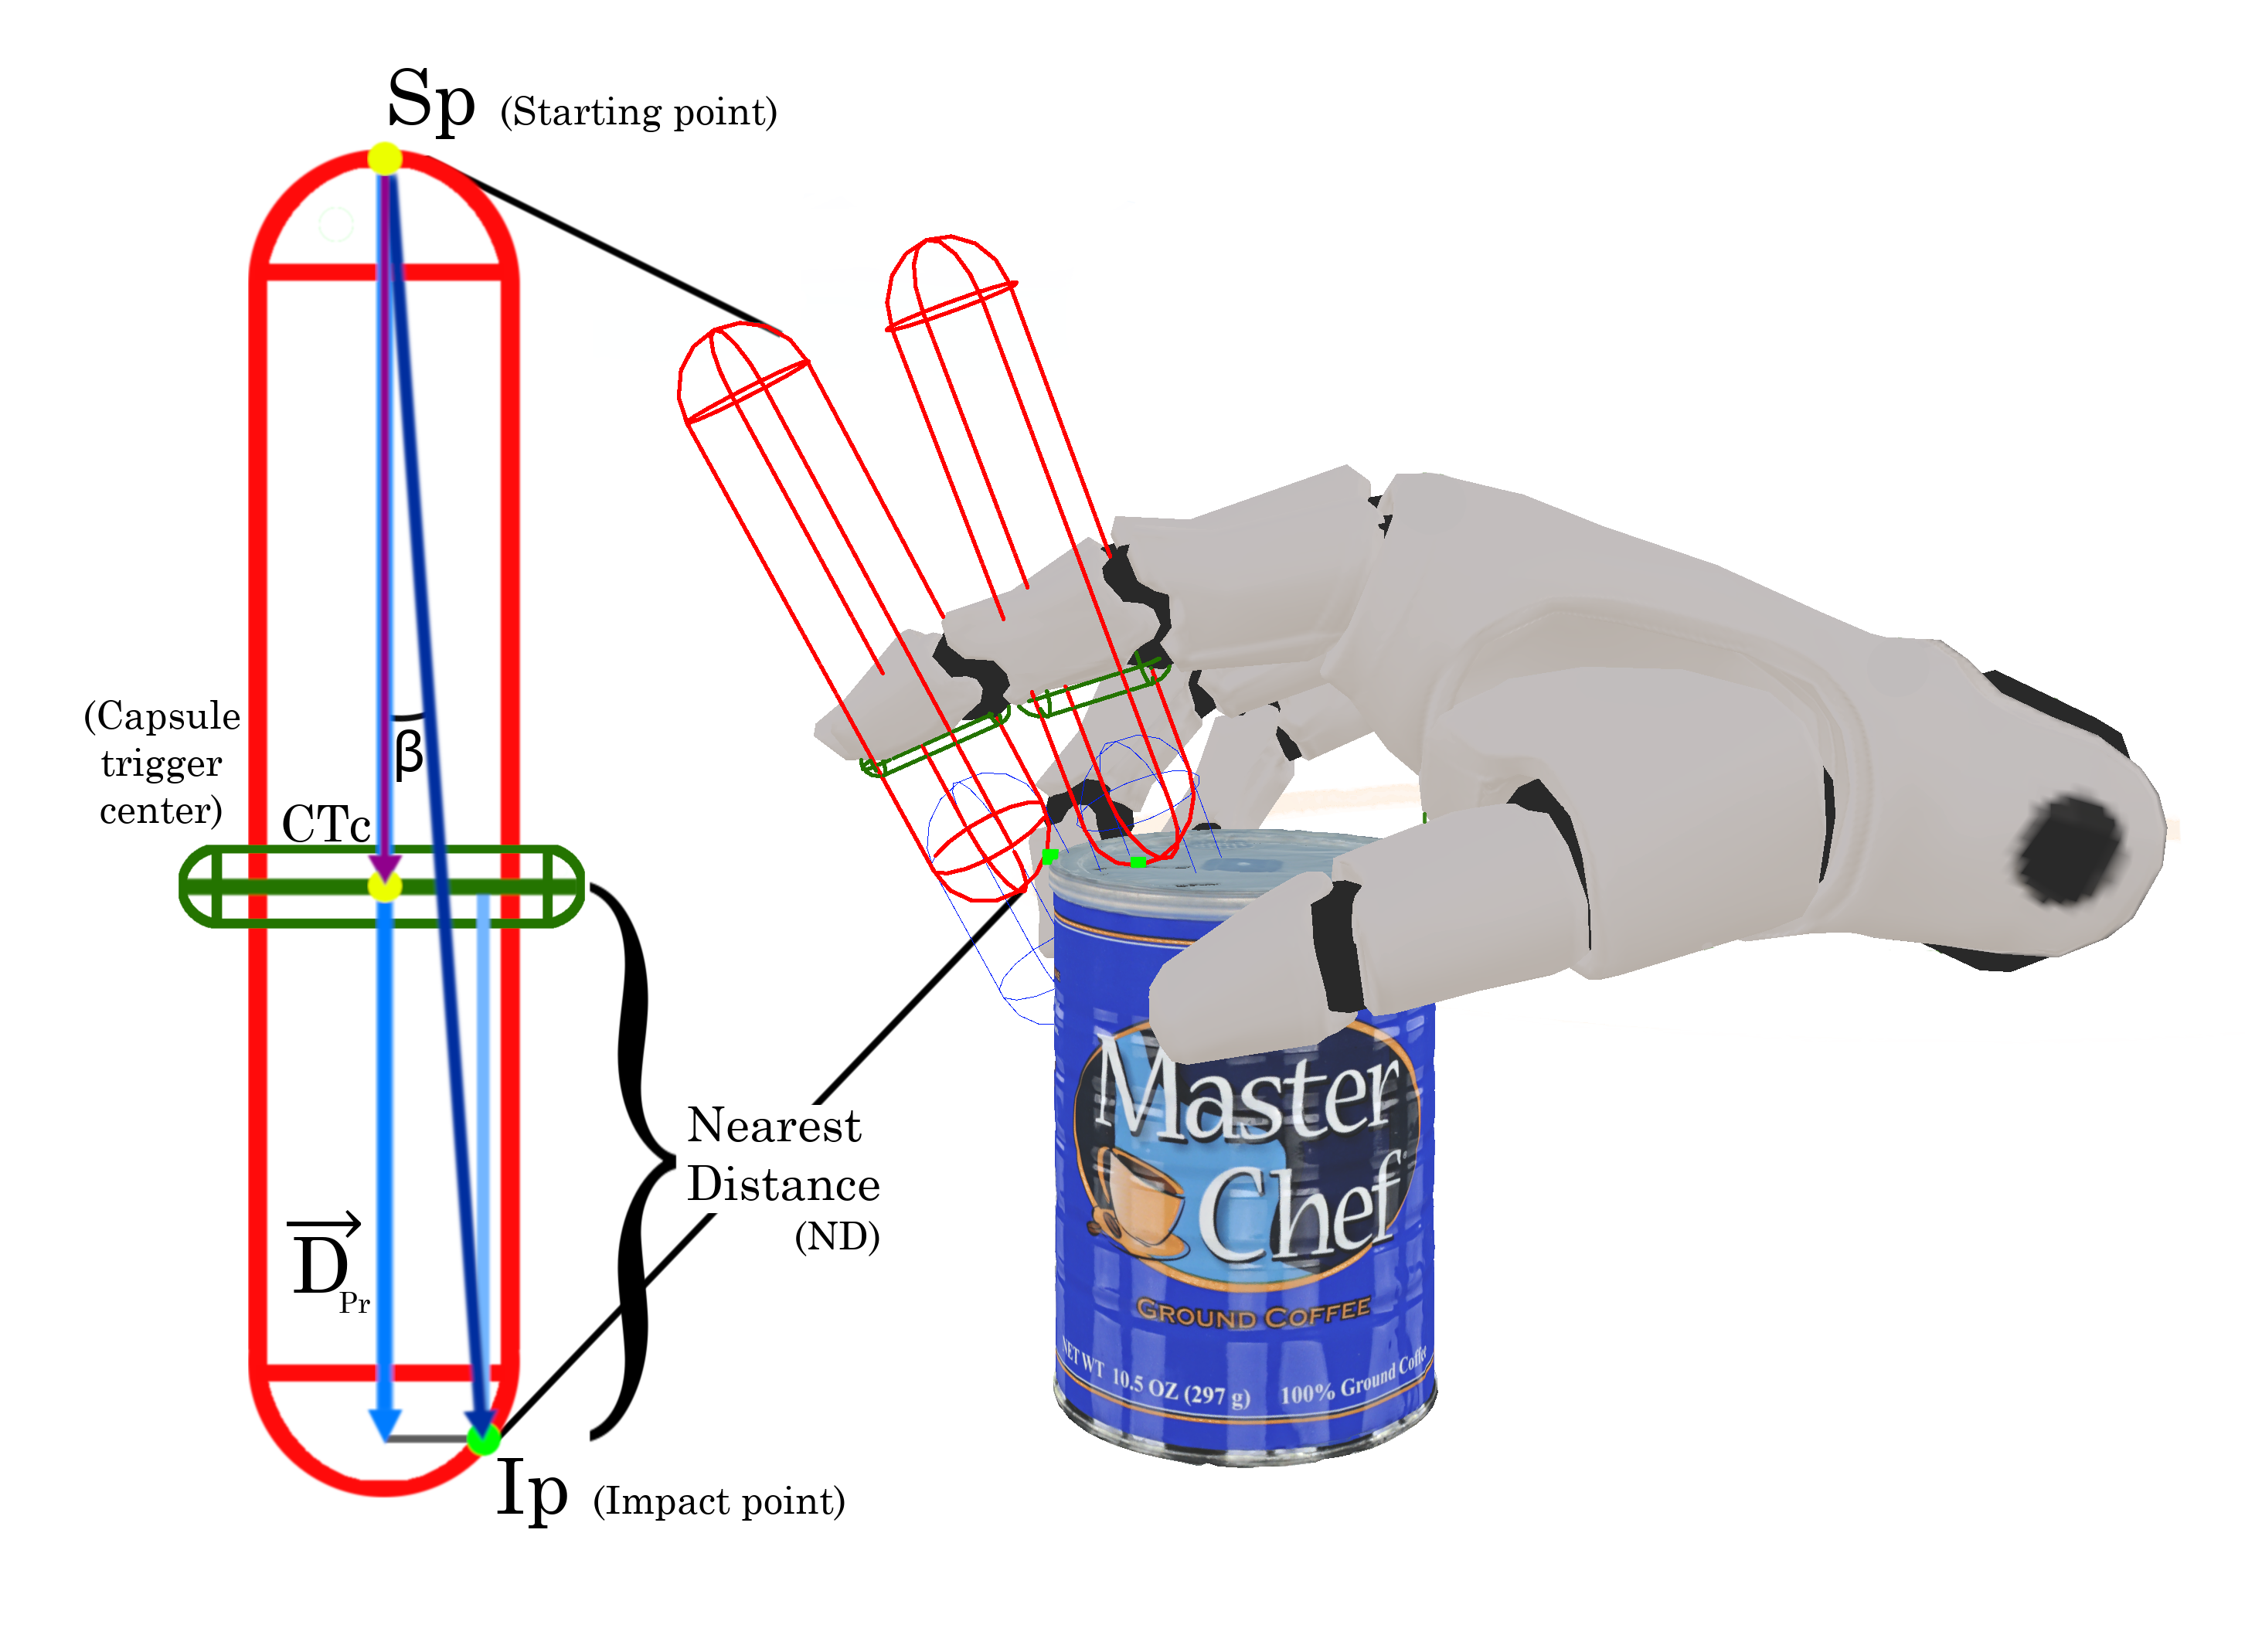
\includegraphics[width=0.70\textwidth]{figures/unrealgrasp/distanceCalculusMod.png}
	\caption{Distance computation for index finger.}
	\label{fig:distanceCalculus}
\end{figure}
The nearest distance computation is approximated by an equation that was developed to find the distance between the impact point, and the plane that contains the capsule trigger center point and is perpendicular to the longitudinal axis of the red capsule. Capsule triggers centers are located on the surface of the hand mesh, so this computation should approximate the nearest distance to the mesh well enough, without being computationally too demanding. To compute this distance, we define the following vectors from the three input points (the starting point of the red capsule, the impact point and the capsule trigger center point):
\begin{equation} \label{eq:1aux1}
\begin{split}
\overrightarrow{D_{Ip}} &= Ip - Sp\\
\overrightarrow{D_{CTc}} &= CTc - Sp
\end{split}
\end{equation}  
where $\overrightarrow{D_{Ip}}$ is the vector from the starting point to the impact point, and $\overrightarrow{D_{CTc}}$ vector represents the direction of the longitudinal axis of the red capsule. They are represented in navy blue and purple respectively in Figure \ref{fig:distanceCalculus}. Then, we find the cosine of the angle they form through their dot product:
\begin{equation} \label{eq:1aux2}
\begin{split}
\overrightarrow{D_{Ip}} \cdot \overrightarrow{D_{CTc}} &= |\overrightarrow{D_{Ip}}| * |\overrightarrow{D_{CTc}}| * cos(\beta)\\
cos(\beta) &= \frac{\overrightarrow{D_{Ip}} \cdot \overrightarrow{D_{CTc}}}{|\overrightarrow{D_{Ip}}| * |\overrightarrow{D_{CTc}}|}\\
\end{split}
\end{equation}
We can now substitute that cosine when computing the projection of $\overrightarrow{D_{Ip}}$ over the longitudinal axis of the red capsule ($\overrightarrow{D_{Pr}}$ in Figure \ref{fig:distanceCalculus}):
\begin{equation} \label{eq:1aux3}
\begin{split}
|\overrightarrow{D_{Pr}}| &= cos(\beta) * |\overrightarrow{D_{Ip}}|\\
|\overrightarrow{D_{Pr}}| &= \frac{\overrightarrow{D_{Ip}} \cdot \overrightarrow{D_{CTc}}}{|\overrightarrow{D_{CTc}}| * |\overrightarrow{D_{Ip}}|} * |\overrightarrow{D_{Ip}}|\\
|\overrightarrow{D_{Pr}}| &= \frac{\overrightarrow{D_{Ip}} \cdot \overrightarrow{D_{CTc}}}{|\overrightarrow{D_{CTc}}|}
\end{split}
\end{equation}
Having that module, we only have to subtract $|\overrightarrow{D_{CTc}}|$ in order to obtain the desired distance:  
\begin{equation} \label{eq:1}
\begin{split}
ND(Ip,Sp,CTc) &= \frac{\overrightarrow{D_{Ip}} \cdot \overrightarrow{D_{CTc}} }{|\overrightarrow{D_{CTc}}|} - |\overrightarrow{D_{CTc}}|\\
ND(Ip,Sp,CTc) &= \frac{\overrightarrow{Ip-Sp} \cdot \overrightarrow{CTc-Sp} }{|\overrightarrow{CTc-Sp}|} - |\overrightarrow{CTc-Sp}|
\end{split}
\end{equation}
Computing the distance like this, with this final subtraction, allows to obtain a positive distance when impact point is outside the hand mesh, and a negative one if it is inside.

We compute the nearest distance per each capsule trigger attached to a finger phalanx. As stated before, if the distance is negative, this indicates a finger penetration issue on the object surface. Otherwise, if distance is positive, it means that finger stopped above the object surface. The ideal case is when a zero distance is obtained, that is, the finger is perfectly situated on the object surface.

The total error for the hand is represented by the following equation:
\begin{equation} \label{eq:2}
HandError = \sum_{i=1}^{N_{Fingers}}\frac{\sum_{j=1}^{N_{CTF}}|ND(Ip_{ij},Sp_{ij},CTc_{ij})|}{N_{CapsuleTriggersPerFinger}}
\end{equation}


\subsection{Procedure}

The system performance analysis begins with the quantitative evaluation. In this first phase, the user will be embodied in a controlled scenario where 30 different objects will be spawned in a delimited area, with random orientation, and in the same order as represented in Figure \ref{fig:ycbgrasps}. The user will try to grasp the object as he would do in real life and as quickly as possible. For each grasping, the system will compute the error metric and will also store the time spent by the user in grasping the object. The purpose of this first phase is to visually analyze grasping quality which is directly related to user expertise in VR environments and concretely with our grasping system. An experienced user would know system limits both when interacting with complex geometries or with large objects that would make it difficult to perform the grasp action quickly and naturally.

For the qualitative evaluation, the same user will be embodied in a photorealistic scenario changing mannequin hands by human hand model with realistic textures. After interacting freely in the photorealistic virtual environment, the user will have to answer the evaluation questionnaire defined in Table \ref{table:questionnaire}. The main purpose is the evaluation of interaction realism, finger and hand movement naturalness and motor control, among other qualitative aspects regarding user experience in VR environments. 

Demo videos for both quantitative and qualitative evaluations are available at Github (\url{https://github.com/3dperceptionlab/unrealgrasp}).


\section{Results and discussion}
\label{sec:results}

In this section we are going to analyze the results obtained from the performance evaluation process represented in Figure \ref{chart:timeanderror}. On one hand, we will draw conclusions on the average time needed to grasp the objects for each user group (experienced and inexperienced) and all users as a whole. On the other hand, we will consider the average error obtained from the interaction with each object. In this way, we will be able to identify the most cumbersome objects to be manipulated, either by their geometry or size. In addition, we will contrast system performance between inexperienced and experienced users to analyze our system behavior with users without previous VR experience.


\subsection{Qualitative evaluation}

Qualitative evaluation for each participant was calculated using the Equation \ref{eq:6} obtaining a score for each qualitative aspect. In Table \ref{table:qualitativeresults} we represent for each group of participants: the average score for each evaluation aspect and the total embodiment score computed using the Equation \ref{eq:5}.

\begin{table}
	\resizebox{0.95\linewidth}{!}{
		\begin{tabular}{lcc}
			\hline
			& \multicolumn{2}{c}{Score} \\
			\cline{2-3}
			Evaluation Aspects    & Experienced users & Inexperienced users \\
			\hline
			(1) Motor Control     & 1.85    & 2.34      \\
			(2) Finger Movement Realism & 2.33   & 2.51       \\
			(3) Interaction Realism      & 1.84     & 1.95      \\
			\hline
			Embodiment score & 1.97 &  2.19 \\
			\hline
	\end{tabular}}
	\caption{Average score for each qualitative aspect of the evaluation and group of participants. Maximum result would be three. Results were obtained using the Equation \ref{eq:6}.}
	\label{table:qualitativeresults}
\end{table}

Regarding the represented results in Table \ref{table:qualitativeresults}, the evaluation of experienced users has been more disadvantageous as they have a more elaborated criterion given their previous experience with virtual reality applications. Finger movement realism (aspect 2) was evaluated similarly by both groups. This is because the hand closing and opening gestures are guided by the same animation in both cases. Finally, the reported results referring to the interaction realism have been the lowest in both cases. This is mostly because users cannot control their individual fingers movement, since general hand gesture is controlled by a unique trigger button of the controller. The average embodiment score computed using the Equation \ref{eq:5} is 2.08 (range of [-3,3]).

\begin{landscape}
	\begin{figure}
		\centering
		\begin{tikzpicture}[baseline]
		\begin{axis}[
		ybar= 0pt,
		xtick=data,
		symbolic x coords= {a,b,c,d,e,f,g,h,i,j,k,l,m,n,o,p,q,r,s,t,u,v,w,x,y,z,aa,ab,ac,ad},
		x tick label style={anchor=north},
		typeset ticklabels with strut,
		enlarge x limits=0.025,
		enlarge y limits=0.3,
		bar width=0.42 em,
		grid=both,
		grid style={line width=.1pt, draw=gray!10},
		major grid style={line width=.2pt,draw=gray!50},
		ylabel={Time [$s$]},
		ylabel near ticks,
		width=\linewidth,
		height=6cm,
		legend style={legend cell align=left, align=left, draw=white!15!black, legend columns= -1},
		legend pos=north west
		]
		\addplot[azure, fill=azure!40] table[x=object,y=0]{data/time_per_object.dat};
		\addplot[red, fill=red!40] table[x=object,y=1]{data/time_per_object.dat};
		\addplot[green, fill=green!40] table[x=object,y=0]{data/time_per_object_overall.dat};
		\legend{Experienced users, Inexperienced users, All users}
		\end{axis}
		\end{tikzpicture}
		
		\begin{tikzpicture}[baseline]
		\begin{axis}[
		ybar= 0pt,
		xtick=data,
		symbolic x coords= {a,b,c,d,e,f,g,h,i,j,k,l,m,n,o,p,q,r,s,t,u,v,w,x,y,z,aa,ab,ac,ad},
		x tick label style={anchor=north},
		typeset ticklabels with strut,
		enlarge x limits=0.025,
		enlarge y limits=0.05,
		bar width=0.42 em,
		grid=both,
		grid style={line width=.1pt, draw=gray!10},
		major grid style={line width=.2pt,draw=gray!50},
		ylabel={Error [$mm$]},
		xlabel={Object [$id$]},
		xlabel near ticks,
		ylabel near ticks,
		width=\linewidth,
		height=6cm, 
		legend style={legend cell align=left, align=left, draw=white!15!black, legend columns= -1},
		legend pos=north west
		]
		\addplot[azure, fill=azure!40] table[x=object,y=0]{data/accuracy_per_object.dat};
		\addplot[red, fill=red!40] table[x=object,y=1]{data/accuracy_per_object.dat};
		\addplot[green, fill=green!40] table[x=object,y=0]{data/accuracy_per_object_overall.dat};
		\legend{Experienced users, Inexperienced users, All users}
		\end{axis}
		\end{tikzpicture}
		\caption{Average time (top) needed to grasp each object and average error (bottom) of the performed grasps. The group of experienced users (i.e. users who had already used virtual reality technologies) is represented in blue, the group of inexperienced users (i.e. users without any previous experience with virtual reality environments) is represented in red, and finally the average time for all users is represented in green.}
		\label{chart:timeanderror}
	\end{figure}
\end{landscape}

\subsection{Quantitative evaluation}

As expected, inexperienced users have taken longer to grasp almost all the objects due to the lack of practice and expertise with the system. Analyzing Figure \ref{chart:timeanderror}, experienced users only have taken longer in grasping some tools such as, the flat screwdriver (Figure \ref{fig:flatscrewdriver}) and hammer (Figure \ref{fig:hammer}). Inexperienced users took an average of 0.36 seconds longer to grab the objects. In practice and regarding interaction, this is not a factor that is going to make a difference. Moreover, the tuna fish can (Figure \ref{fig:tunafishcan}), potted meat can (Figure \ref{fig:pottedmeatcan}), spatula (Figure \ref{fig:spatula}), toy airplane (Figure \ref{fig:toyairplane}) and bleach cleaner (Figure \ref{fig:bleachcleaner}) are the most time consuming when grasped by the users. This is mainly because of their sizes and complex geometries. Since objects are spawned with a random orientation and taking into account that, for example, the power drill (Figure \ref{fig:powerdrill}) and spatula have a handle, the time needed to grasp them can be variable and also related to the user VR skills. The user would unconsciously try to grasp the object by its handle, which would add some extra time depending on the orientation of the handle relative to the hand when the object is spawned. Even so, we can conclude that generally the largest objects are those that the user takes the longest to grasp.

Analyzing the average error obtained for each object, a similarity is observed between the results of inexperienced users and those experienced. The most significant differences were observed when manipulating the power drill and the spatula. This is because its complex geometries and large dimensions make it difficult to grasp (as in the case of toy airplane). Analyzing also the overall error, we come to the conclusion that the largest objects, such as the toy airplane, power drill, and bleach cleaner are those with the highest error rate. In addition, we observe how overall error decreases in time from the first object manipulated to the last. This is mainly because, user skills and expertise with the grasping system are improving progressively. On the basis of the obtained results, we can conclude that our solution is user-friendly, a fact that refers to a steep learning curve.


\section{Applications}
\label{sec:applications}

Our grasping system can be applied to several existing problems in different areas of interest, such as: robotics \cite{bric2016current}, rehabilitation \cite{levin2015emergence} and interaction using augmented reality \cite{lv2015touch}.

In robotics, different works have been explored to implement robust grasp approaches that allow robots to interact with the environment. These contributions are organized in mainly four different blocks \cite{bohg2014data}: methods that rely on known objects and previously estimated grasp points  \cite{lin2015robot}, grasping methods for familiar objects\cite{vahrenkamp2016part}, methods for unknown objects based on the analysis of object geometry \cite{zapata2017using} and automatic learning approaches\cite{levine2018learning}. Our approach is more closely related to this last block, where its use would potentially be a relevant contribution. As a direct application, our system enables human-robot knowledge transfer where robots try to imitate human behavior in performing grasping.

Our grasping system is also useful for rehabilitation of patients with hand motor difficulties, and it could even be done remotely assisted by an expert \cite {escobar2018virtual}, or through an automatic system \cite{avola2018vrheab}. Several works have demonstrated the viability of patient rehabilitation in virtual environments \cite{levin2015emergence}, helping them to improve the mobility of their hands in daily tasks \cite{faria2016benefits}. Our novel error metric in combination with other automatic learning methods, can be used to guide patients during rehabilitation with feedback information and instructions. This will make rehabilitation a more attractive process, by quantifying the patient progress and visualizing its improvements over the duration of rehabilitation.

Finally, our grasping system integrated in UnrealROX \cite{martinez2019} enables many other computer vision and artificial intelligence applications by providing synthetic ground truth data, such as depth and normal maps, object masks, trajectories, stereo pairs, etc. of the virtual human hands interacting with real objects from the YCB dataset.


\section{Limitations and future works}
\label{sec:limitationsfutureworks}
Our proposal has several major limitations:
\begin{itemize}
	\item Hand movement is based on a single animation regardless object geometry. Depending on the object shape we could vary grasping gesture: spherical-grasping, cylindrical-grasping, finger-pinch, key-pinch, etc. However, our grasping gesture was experimentally the best when dealing with different shaped objects. 
	\item The object can be grasped with only one hand. The user can interact with different objects using both hands at the same time. But not the same object with both hands. 
	\item Sometimes it is difficult to deal with large objects due to the initial hand posture or because objects slide out from the hand palm due to physical collisions. Experienced users can better deal with this problem.
\end{itemize}

As future work, and in order to improve our grasping system, we could vary the hand grip gesture according to the object geometry we are manipulating. This is finding a correspondence between object geometry and a simple shape, e.g. a tennis ball is similar to a sphere thus proceeding with a spherical grasp movement. At the application level, there are several possibilities as we discussed in the previous section. However, we would like to emphasize the use of contact points obtained when grasping an object in virtual reality, to transfer the human behavior to real robots.


\section{Conclusions}
\label{sec:conclusion}
This work proposes a flexible and realistic looking grasping system which enables smooth and real-time interaction in virtual reality environments with arbitrary shaped objects. This approach is not restricted by object geometry, is fully user-controlled, and is modular and easy to implement on different meshes or skeletal configurations. In order to validate our approach, an exhaustive evaluation process was carried out. Our system was evaluated qualitatively and quantitatively by two groups of participants: with previous experience in virtual reality environments (experienced users) and without expertise in VR (inexperienced). For the quantitative evaluation, a new error metric has been proposed to evaluate each grasp, quantifying hand-object overlapping. From the performance analysis results, we conclude that user overall experience was satisfactory and positive. Analyzing the quantitative evaluation, the error difference between experienced users and non experienced is subtle. Moreover, average errors are progressively smaller as more object are grasped. This clearly indicates a steep learning curve. In addition, the qualitative analysis points to a natural and realistic interaction. Users can freely manipulate previously defined dynamic objects in the photorealistic environment. Moreover, grasping contact points can be easily extracted, thus enabling numerous applications, especially in the field of robotics. Unreal Engine 4 project source code is available at GitHub alongside several video demonstrations (\url{https://github.com/3dperceptionlab/unrealgrasp}). This approach can easily be implemented on different game engines.